\documentclass[11pt,a4paper]{report}
\usepackage[latin1]{inputenc}
\usepackage[T1]{fontenc}
\usepackage[english]{babel}
\usepackage{eso-pic}
\usepackage{graphicx}
\usepackage{geometry}
\usepackage{amsmath}
\usepackage{pgfgantt}
%\usepackage{tikz}
\usepackage{float}
\usepackage{url}
\usepackage{hyperref}
\usepackage[nottoc]{tocbibind}
\usepackage{algorithm2e}
\usepackage{longtable}
\usepackage{eurosym}
\usepackage{listings}
\usepackage{subfigure}
\usepackage{comment}
\usepackage{slashbox}
\usepackage[nopostdot, nonumberlist]{glossaries}


\newcommand{\backgroundpic}[3]{
  \put(#1,#2){
    \parbox[b][\paperheight]{\paperwidth}{
      \centering
 \includegraphics[width=\paperwidth,height=\paperheight,keepaspectratio]{#3}
      \vfill
}}}

\def\keywords#1{\begin{center}{\bf Keywords}\\{#1}\end{center}}

\lstdefinestyle{erlang}{
   language        = erlang,
   showstringspaces= false,
   breaklines      = true,
   keywordstyle    = {\bfseries},
   keywordstyle    = [2]{\color{green}},
   keywordstyle    = [3]{\color{red}},
   alsoletter      = {?, :},
   morekeywords    = {
     new,
     fun,
     begin},
   morekeywords    = [2]{
     ?FORALL,
     ?LET},
   morekeywords    = [3]{
     eqc:numtests,
     eqc:quickcheck,
     eqc_c:start,
     eqc\_statem:show\_states,
     car,
     car\_xml}
}
\lstdefinestyle{c}{
  language        = c,
  commentstyle    = \color{purple},
  keywordstyle    = \color{violet},
  showstringspaces= false
}
\lstdefinestyle{autosar}{
  breaklines      = false,
  frame           = l,
  showstringspaces= false,
  string          = [s]{``}{''},
  morestring      = [b]",
  basicstyle      = \color{red},
  keywordstyle    = \color{blue},
  commentstyle    = \color{green},
  stringstyle     = \color{green},
  moredelim       = [is][\color{cyan}]{|}{|},
  literate        = {<=}{{$\leq$}}{1} %% observe no comma
                    {>=}{{$\geq$}}{1},
  identifierstyle = \color{black},
  emph            = {
    WdgMExpiredSupervisionCycleTol,
    WdgM_MainFunction,
    WdgM_SetMode,
    WdgM_Init,
    WdgM_DeInit,
    WdgM_CheckpointReached,
    WdgM_CalculateAliveSupervision,
    WdgM_CheckLogicalSupervisedEntities
  },
  emphstyle       = {\color{cyan}},
  morekeywords    = {
    WDGM\_CORRECT,
    WDGM\_INCORRECT,
    WDGM\_GLOBAL\_STATUS\_OK,
    WDGM\_GLOBAL\_STATUS\_FAILED,
    WDGM\_GLOBAL\_STATUS\_EXPIRED,
    WDGM\_GLOBAL\_STATUS\_STOPPED,
    WDGM\_GLOBAL\_STATUS\_DEACTIVATED,
    WDGM\_LOCAL\_STATUS\_OK,
    WDGM\_LOCAL\_STATUS\_FAILED,
    WDGM\_LOCAL\_STATUS\_EXPIRED,
    WDGM\_LOCAL\_STATUS\_DEACTIVATED
  }
}

\makeglossaries
% \newglossaryentry{WdgM}
% {
%   name=WdgM,
%   description={Watchdog Manager, a module which supervises the execution
%                of basic software components.}
% }

\newacronym{ECU}{ECU}{Electronic control unit.}
\newacronym{Wdg}{Wdg}{Watchdog (the hardware).}
\newacronym{WdgIf}{WdgIf}{Watchdog Interface.}
\newacronym{WdgM}{WdgM}{Watchdog Manager.}
\newacronym{SF}{Supervision functions}{Logical-, Deadline or Alive supervision.}
\newacronym{SE}{Supervised Entity}{A critical section in the supervised program.}
\newacronym{CP}{Checkpoint}{A point in the supervised entity. These points can be configured and used for different supervision functions.}
\newacronym{ASIL}{ASIL}{Automotive safety integrity level.}
\newacronym{Positive}{Positive testing}{Trying to stay in a valid good state when testing by generating valid input data and command sequences.}
\newacronym{Negative}{Negative testing}{Testing that, when generating negative/invalid input data or invalid command sequences, should raise errors.}

\begin{document}
\pagenumbering{Alph}
% Chalmers title page
\begin{titlepage}

  \AddToShipoutPicture{\backgroundpic{-4}{56.7}{frontpage.pdf}}
  \mbox{}
  \vfill
  \addtolength{\voffset}{2cm}
  \begin{flushleft}
    {\noindent {\huge Evaluation of validity of verification methods:} \\
      {\huge Automating functional safety with QuickCheck} \\
      \emph{\Large Master of Science Thesis} \\[.8cm]

      {\huge Oskar Ingemarsson}\\
      {\huge Sebastian Weddmark Olsson}
      \vfill
      {\normalsize Chalmers University of Technology \\
        University of Gothenburg \\
        Department of Computer Science and Engineering \\
        Gothenburg, Sweden, September 2013 \\
      }
    }
  \end{flushleft}

\end{titlepage}
\ClearShipoutPicture
% End Chalmers title page
\pagenumbering{gobble}

\vspace*{2.5cm}
The Author grants to Chalmers University of Technology and University of Gothenburg  the non-exclusive right to publish the Work electronically and in a non-commercial purpose make it accessible on the Internet.\\
The Author warrants that he/she is the author to the Work, and warrants that the Work does not contain text, pictures or other material that violates copyright law. \\

The Author shall, when transferring the rights of the Work to a third party (for example a publisher or a company), acknowledge the third party about this agreement. If the Author has signed a copyright agreement with a third party regarding the Work, the Author warrants hereby that he/she has obtained any necessary permission from this third party to let Chalmers University of Technology and University of Gothenburg  store the Work electronically and make it accessible on the Internet.\\[0.6cm]

{\setlength{\parindent}{0cm}


  {\Large Evaluation of validity of verification methods:}\\
  {\large Automating functional safety with QuickCheck}\\

  {OSKAR INGEMARSSON}\\
  {SEBASTIAN WEDDMARK OLSSON}\\

  \copyright ~OSKAR INGEMARSSON, September 2013.\\
  \copyright ~SEBASTIAN WEDDMARK OLSSON, September 2013.\\

  Examiner: MENG WANG\\
  Supervisor: JOSEF SVENNINGSSON\\

  Chalmers University of Technology\\
  University of Gothenburg\\
  Department of Computer Science and Engineering\\
  SE-412 96 G\"{o}teborg\\
  Sweden\\
  Telephone + 46 (0)31-772 1000\\
  \vfill
  % \{Cover:\\
  % an explanatory caption for the (possible) cover picture\\
  % with page reference to detailed information in this essay.\}\\

  Department of Computer Science and Engineering\\
  G\"{o}teborg, Sweden, September 2013
}
\newpage
\pagenumbering{roman}

\pagenumbering{roman}

\begin{abstract}
Abstract is often proportional to the thesis length.

\keywords{AUTOSAR, Semi formal verification, QuickCheck}
\end{abstract}
\setcounter{page}{2}
\tableofcontents

\glsaddall
\printglossary

\clearpage

\pagenumbering{arabic}
\chapter{Introduction}
% In the first sections of this chapter we outline the background, purpose and
% objectives and the last section describes the scope of our research. Chapter 2
% contains the theory needed for understanding the thesis, existing software and
% some verification methods described in the standards. Methods is described in
% Chapter 3 and the results in Chapter 4. In Chapter 5 and 6 we have a discussion
% and some conclusions about the results.

%Background to the assignment. Why is it relevant?
\section{Background}
\subsection{The Development within automotive industry}
In the recent decades there has been a dramatic growth of information and
communication innovations within the automotive industry
\cite{CRC:embedded_handbook}. Analog vehicles have been transformed into complex
electromechanical systems \cite{Cambridge:controlsystems}. New features are
implemented (for example due to user demands, traffic safety or environmental
regulations \cite{Springer:advanced_microsystems}\cite{ISO26262}) requiring more
computational power and less energy consumption
\cite{Springer:advanced_microsystems}. The average car has already 80 ECU's
(electronic computation units)
\cite{Springer:advanced_microsystems}\cite{QUVIQ:COURSE} and to deal with
the extra functionality, each ECU will need to
become more complex \cite{Springer:advanced_microsystems}.%  This could be done
% with the use of multicore ECU's, which can provide more computational power in a
% more energy effective way \cite{Springer:advanced_microsystems}.

\subsection{Extent of software in modern vehicles}
Developing a new car model costs up to one billion \euro
\cite{Clemens:tech_acceptance}, where electronics has reached a mean share of
one third of the value, divided 20\% sensor value, 40\% hardware value and 40\%
software value \cite{Wiley:internetworking}. The share of software has been
doubled the last 10 years \cite{Wiley:internetworking}.

More and more functions will be implemented; Intelligent traffic systems which
make the automotive vehicles communicate \cite{VOLVO:convoys} with the roadside management systems
\cite{Cambridge:controlsystems}, infotainment systems will bring, among other,
weather information through the Internet and emergency call support
\cite{Wiley:internetworking}\cite{Springer:advanced_microsystems}, traffic sign
recognition \cite{Springer:advanced_microsystems}, night vision
\cite{Wiley:internetworking}\cite{Springer:advanced_microsystems} and automated
parking \cite{Springer:advanced_microsystems}.

The number of lines of code running in a vehicle is another example of how
complex the automotive software is. The software running on a F-22 Raptor
and the F-35 Strike Fighter, two of the attack planes in the US air force, has
about 1.7 million lines of code and 5.7 million lines of code respectively
\cite{IEEESpectrum:car_code}. The passenger plane Boeing 787 Dreamliner runs on
6.5 million lines of code, where the average premium-class car has close to 100
million lines of code \cite{IEEESpectrum:car_code}.

\subsection{Introduction of standards}
Because of the high development costs, and the complexity of modern cars, car
manufacturers, suppliers and other companies related to the automotive industry
joined efforts in 2003 and created AUTOSAR, short for Automotive Open System
Architecture \cite{AUTOSAR:basic_info}. The main purpose is to make it possible
for car manufacturers to buy independent components from different software
suppliers; the AUTOSAR motto is ``Cooperate on standards, compete on
implementation'' \cite{AUTOSAR:basic_info}.

Functional safety was introduced to the automotive industry with ISO 26262 in
late 2011 \cite{ISO26262}. ISO 26262 named ``Road vehicles -- Functional safety''
is a general standard on how the implementation of functional safety in vehicle
development should be carried out from beginning to end \cite{ISO26262}.

This standard is built on top of another industrial standard IEC 61508
\cite{ISO26262}, named ``Functional safety of electrical/electronic/programmable
electronic safety-related systems'' \cite{IEC61508}, which purpose is to ensure
functional safety in computer based systems' overall life cycles
\cite{IEC61508}.

It is useful to distinguish between systems with different levels of
dependability, and determine where the hazards
exists\cite{COURSEBOOK:safety-critical}. When this risk analysis is completed,
and appropriate reliability and availability requirements is assigned to the
system, the system can be identified by a certain safety integrity level (SIL).
If this number is high, the system will experience a more rigorous design and
testing than could be justified for a lesser demanding system. These levels are
more defined in the standards IEC~61508 and ISO~26262.



\subsection{Testing}
Functional safety demands testing \cite{ISO26262}, and testing accounts for
around half of all software development costs
\cite{QUICKCHECK:lightweight}\cite{QUICKCHECK:software}. Reducing the cost is
motivated and can be done by automating the test generation process
\cite{QUICKCHECK:software}\cite{Testing:black_box}.

For simple devices it is possible to exhaustively test the functional safety of
the system \cite{COURSEBOOK:safety-critical}. For example consider system
consisting of a small number of switches, where each switch has only two states;
open and closed. Then the number of possible failures can be determined by the
combination of all possible failure states of each individual switch. The
complexity issue is that in systems such as microprocessors or ECU's, the
number of possible failure states is so large that it is considered
infinite. This makes it impossible exhaustively test the system, and therefore,
make the detection of failures unreliable.

%Aim for the work. What should be accomplished?
\section{Purpose}
The purpose is to automate the testing process of automotive software in an
effective and good way and to make it possible to raise the Automotive Safety
Integrity Level (ASIL), where applicable.

It is desired to do an evaluation of tools that can be used in order to perform
at least semi formal verification of automotive software modules. The main
purpose is however to evaluate if Quviq QuickCheck can be used to fulfill this.

%question formulation?
%The problem at hand, the assignment
\section{Objective}
The first problem at hand is to evaluate what ``semi formal verification'',
according to the ISO-standard, means. In formal methods of mathematics, formal
verification means to prove the correctness of algorithms.
The ISO-standard mentions both ``formal verification'' and ``semi
formal verification'' for software development, but does not describe how to
achieve any of these.
This evaluation must be done to get knowledge of how to properly implement
functional safety and reach an ASIL classification, using automated testing.

%The second problem is to evaluate if QuickCheck can be used to achieve this.
%QuickCheck grants the ability to automate the testing, and knowledge of this
%ool exist in the corporation where this thesis is done. %% F�retaget hm....

A model for an AUTOSAR module needs to be implemented. For this to be a good
model some questions first needs to be answered.
How can one achieve good test cases for the model? How can one tweak the test
generation to find test cases that are interesting in a safety critical point of
view? Is the implemented model together with the generated tests good enough to
reach the goals?

The test generation is a big problem when verifying a model. With unit tests, one
can argue for that each line of code has been executed (100\% code coverage),
but that is just a statement for that everything has been executed. Have it been
executed correctly?
Are every combination of computations in the system necessary to ensure
correctness, or with other words, is it possible to collapse some states in the
system's state space without endangering the safety of the hole system?

After the model has been implemented, there must be an evaluation of the
solution. Does it ensure functional safety? How can one measure the
size of the state space that is actually verified?
Even if test generation has been done properly, the solution might not be within
the ISO-standards means of functional safety.

One must propose and motivate what should be done to be able to
achieve a semi formal verification. This can include a confidence interval
for how certain the verification is. The confidence interval would help
describing the visited state space because it is probably not feasible to
exhaustively visit all states due to the state space explosion problem.

The main objective is to prove that it is possible to do semi formal
verification for an AUTOSAR module and its specification.
It should not matter which configuration that is active and even further
how the module is implemented, because the specification should hold for all
configurations and implementations. This gives rise to that every company that
implements the module should be able to run the final code to achieve ``semi
formal verification''. Since modules in AUTOSAR are dependent, the work
presented here should be generalized so it can be hooked on when implementing
test suits, using the same techniques, for other modules.

%Limitations. What should be left out and why?
\section{Scope}
We will use AUTOSAR 4.0 revision 3 for our thesis work.
Since this version of AUTOSAR consists of more than 100 specifications and other
auxiliary materials\cite{AUTOSAR:URL}, we will limit our scope to one
specification. The module of this thesis is the Watchdog Manager. This
module provides monitoring services used to maintain correctness. The
module is chosen because it got dependencies, and is used to report
development and production errors, but mainly because it executes
safety-critical work. The fact that it got dependencies is important when doing
integration testing.

The aim of the work is also to verify software components. In other words no
work considered hardware or a combination of hardware and software will be
prioritized. All implemented code for the verification will run on a standard
PC-machine.

%% l�gga till ett stycke ang�ende att vi bara g�r in p� 6-9 och 6-10, och inte
%% p� 6-8 eller 6-11.

We will not implement deprecated API-functions in our model, nor will we test
configurations which will give raise to segmentation faults.

%% skriva n�got om varf�r vi inte vill testa segmentation fault configs?

\chapter{Theory}
\section{Verification}
The exact meaning of verification is confusing \cite{thomas_arts}. The
definition may differ in comparison of academic or industrial use. Even in
different phases of the safety life cycle verification is conducted in various
forms \cite[8:9.2]{ISO26262}.

\subsection{Formal Verification}
%Skriv n�got luddigt
Formal verification is very hard to achieve for software, due to the state space
explosion problem. To achieve formal verification, one must visit every state
that exists, and prove for each of those states, that the code is correct. State
space explosion occur when a small increase of elements rapidly raises the
number of combinations to a computational maximum. %% SKRIV OM!!!!!!!!!!!
                                %% framf�r allt sista meningen men ocks� binda
                                %% ihop med ISO~26262 och "state-space
                                %% complexity"

\subsection{Semi formal verification}
%Skriv n�got �n mer luddigt
Semi formal verification covers a smaller state space than formal
verification.

\section{Industrial Standards} It is useful to distinguish between
systems with different levels of dependability, and determine where the hazards
exists\cite{COURSEBOOK:safety-critical}. When this risk analysis is completed,
%% �verv�g kommatecken mellan dessa satser
and appropriate reliability and availability requirements is assigned to the
system, the system can be identified by a certain safety integrity level (SIL).
If this number is high, the system will experience a more rigorous design and
testing than could be justified for a lesser demanding system. These levels is
more defined in standards IEC~61508 and ISO~26262.

%\section{Functional Safety}
% Kanske n�got vi vill skriva om? N�ms i metoden

\subsection {IEC~61508 and ISO~26262}

%% SKRIV OM IEC~61508

%G�r skillnad p� verifikation och verifikation. Dvs vilken fas handlar det om?
Automotive software for safety related systems is required to be designed,
implemented and verified by the standard ISO~26262, which handles functional
safety for automotive equipment. For a higher level of integrity ISO~26262
strongly recommends that semi formal verification of each module should be
executed \cite[Part 6]{ISO26262}. It also recommends a formal verification, but
because of the state-space complexity this is hard to achieve.

%% Skriv om integrationstester mot unittester etc, (6-9, 6-10, 6-11 i ISO)

ISO~26262 describes the full development process from concept to production,
with functional safety in mind. For software development, the standard has a
reference model with different phases of the process, see
figure~\ref{FIG:ISO:phases}. Each phase in the reference model is dependent on
the earlier phases. The reference model has the shape of a V, where the left
side contains all development phases, and the right side contains the test
phases. The work flow from this view starts with the phase ``specification of
software safety requirements''. This phase specifies the software requirements
needed to ensure the stability of the system. They are derived from the
system design specification. This is part of the integration between software
and hardware. The second phase is the ``software architectural design''. It
represent the interaction between all software components. The third phase and
the last development phase, in the model is the ``software unit design and
implementation''. This phase contains the implementation of each module. If the
implementation does not meet the wished safety, maybe the software
architectural design or the specification of the software safety requirements
need to be redesigned.

\begin{figure}
  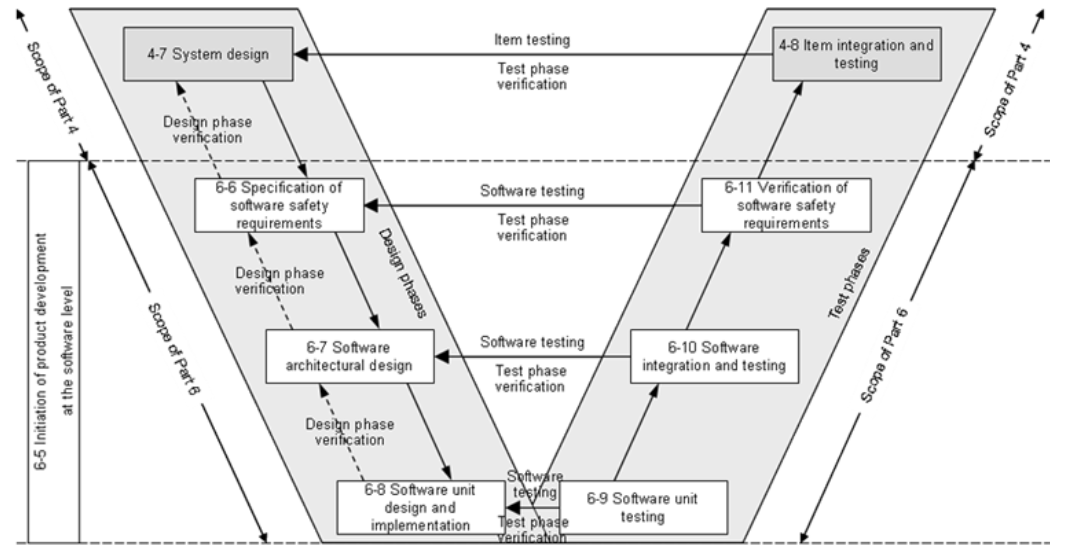
\includegraphics[keepaspectratio, width=\linewidth]{pictures/V}
  \caption{Phases of software development in the standard ISO~26262}
  \label{FIG:ISO:phases}
\end{figure}

Each of these phases is tested thoroughly with the phases ``software unit
testing'', ``software integration and testing'' and ``verification of software
safety requirements''. The unit testing phase tests that the implementation of
the module fulfills the design specifications. If there is failures, one need to
go back to the implementation phase, or if successful go to the phase
integration and testing. This phase objective is to integrate the software units
and demonstrate that the architectural design is correct. A demonstration that
the software safety requirements is fulfilled, is done in the phase
``verification of software safety requirements''.

% ISO~26262 is built on IEC~61508 which is titled Functional Safety of
% Electrical/Electronic/Programmable Electronic Safety-related Systems. IEC~61508
% can be applied to any kind of industry while ISO~26262 is defined only for the
% automotive industry. IEC~61508 have four safety integrity levels (SIL) ranked
% 1-4. SIL 4 is the highest and should be applied where a failure can
% do devastating damage to a large area. %% �r det inte ocks� s� att om det �r
%% ganska farligt men riskerar att h�nda ofta s� ska den ocks� klassas som SIL
%% 4.

\subsection{AUTOSAR (AUTomotive Open System ARchitecture)}
%K�lla http://www.autosar.org/
The AUTOSAR platform has a layered software architecture. This means that the
architecture is divided to a number of different layers, such as the application
layer, runtime environment, the basic software layer, and the
microcontroller. In the Figure~\ref{FIG:AUTOSAR:architecture} the basic software
layer is represented as four different parts; services, ECU
abstraction, microcontroller abstraction, and complex drivers.

\begin{figure}[!ht]
  \begin{center}
    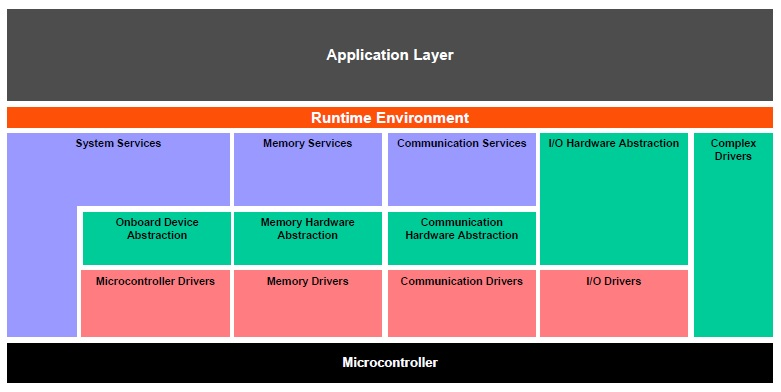
\includegraphics[keepaspectratio, width=\linewidth]{pictures/autosar_architecture.jpg}
  \end{center}
  \caption{The AUTOSAR software architecture. Noticeable is that the basic
    software layer is divided further into three categories with more subsections.}
  \label{FIG:AUTOSAR:architecture}
\end{figure}

The runtime environment is the OS, and the microcontroller is the hardware. The
software running in the application layer is applications such as sensors and
actuators. %% skriva n�got mer om applikationslagret.

%% Saxxat fr�n AUTOSAR Layered software
% Automotive ECUs have the properties: strong interaction with hardware,
% connection to vehicle networks, limited computing power and memory, real time
% system, program execution from internal or external flash memory.

% The AUTOSAR architecture is a generic approach, standard modules can have
% extended functionality and still be compliant.

One example of how the different parts in the basic software layer is
integrated, is the watchdog, which consist of several parts as seen in Figure~\ref{FIG:AUTOSAR:watchdog}. The
microcontroller abstraction layer has the drivers for the watchdog, the
interaction with the microcontroller. Then there is the watchdog interface at
the ECU abstraction layer. The watchdog interface is the onboard device
abstraction. Last is the watchdog manager which runs as a system service in the
service layer.

\begin{figure}[!ht]
  \begin{center}
    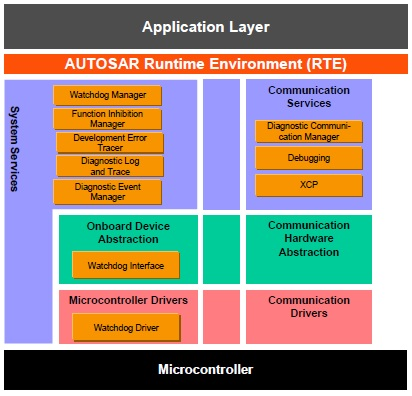
\includegraphics{pictures/watchdog_architecture.jpg}
  \end{center}
  \caption{The Watchdog and some other related modules.}
  \label{FIG:AUTOSAR:watchdog}
\end{figure}

The watchdog have a number of dependencies to other services in the basic
software layer. For example when an error is found by the watchdog, it should be
reported to either the diagnostic event manager or the development error
tracer. Two services used for error management. %% bra eller anus att skriva av
                                %% den ska skicka fel till DEM eller DET n�r vi
                                %% skriver i n�sta avsnitt att det g�r att ta
                                %% bort DEM rapporteringen?

AUTOSARs concept is to make it possible for vehicle manufacturers to buy modules
from different software developers, which will still work together in
unison. For vehicle manufacturers to have different work done by the same
software developer's
module, the standard introduce configurations. There exist a number of variables
to configure. In the watchdog manager, there is for example variables that
specify if the watchdog manager should report errors to the diagnostic event
manager (DEM), or which type of supervision that should be done and what to
supervise.

The current version of AUTOSAR, version 4, has been design with functional
safety in mind. Essential concepts of ISO~26262 have been developed alongside
AUTOSAR.
%% SKRIV MER OM functional safety i version 4 av AUTOSAR


% Some of the specifications in AUTOSAR is left quite open for interpretation.
% %% beskriv varf�r dessa inte �r tillr�ckligt definierade, och varf�r olika
% %% konfigurationer existerar.
% This makes it possible for vehicle developers to have different specifications
% for a configuration. Some parts of those configuration specifications is
% generated into code, while other is manually written or added as a configurable.

\subsection{QuickCheck}
QuickCheck was invented be Koen Claessen and John Hughes, as a testing module
for Haskell, in 2000.
In 2006 John Hughes founded the Company Quviq together with
Thomas Arts\cite{QUVIQ:about}. Quviq offers a commercial version of QuickCheck for Erlang.
The main difference, except from the programming paradigms, is that
the commercial version of QuickCheck has a C-testing interface. Hence it
possible to test C-code in Erlang with help of QuickCheck. All code for tests
is written in Erlang and checked against API calls to the C-code. It is actually
not necessary to have actual source code; it is enough to only have compiled library
files.

QuickCheck tests a program with specification implemented as properties that
the program must hold \cite{QUICKCHECK:manual}. QuickCheck has guided random
test generation, this means that the samples can be weighted to cover certain
parts of the state-space with more likelihood.

\section{Verification Methods}
The standard IEC~61508 propose two methods to say that a program is formal
verified. The key is to model the program into one of the following machines.

\begin{enumerate}
\item \label{enum:FSM} Finite state machines/state transition diagrams
\item Time Petri nets
\end{enumerate}

IEC~61508 emphasises that Time Petri nets are best suited for concurrent
programs. Regarding method \ref{enum:FSM} the following criteria needs to be
satisfied for the implemented state machine to be formal verified:

\begin{description}
\item[completeness] the system must have an action and new state for every input
in every state,
\item[consistency] only one state change is described for each state/input
pair, and
\item[reachability] whether or not it is possible to get from one state to
another by any sequence of inputs.
\end{description}

If the state machine is correctly implemented it exist a correct model of the
%% det �r n�got konstigt med denna meningen men jag kan inte riktigt s�tta
%% fingret p� det.
%% kan vara att: om SM �r korrekt implementerad - s� �r originalprogrammet
%% formellt verifierat. �r detta verkligen allt som kr�vs?
original program, then the original program is formal verified.

Since most program specification are written in natural languages there may be
lots of ambiguities. Consequently a lot of techniques has been developed to reduce
such cases. These techniques are often referred to as semi formal verification,
because they lack of mathematical rigour associated with formal
verification. These methods use textual, graphical or other notation; often
several techniques are used in unity. % These tests may not be

The description of semi formal verification in IEC~61508 states: \\
''Semi-formal methods provide a means of developing a description of a system at
some stage in its development, i.e. specification, design or coding. The
description can in some cases be analysed by machine or animated to display
various aspects of the system behaviour.''


\chapter{Method}
%% kolla att allt �r i imperfekt
%% verb i passiv form

\section{Existing verification tools}
Software unit testing can be achieved by almost any tool.
%% motivera.
Consequently this phase is not the most interesting when it comes to the choice
of a tool verification. Of course one can take the simplicity to achieve good
%% "simplicity" - av vad?
unit testing into account, but still it is not what makes a verification tool
especially unique for the project goals.

Since the purpose is about benchmarking software the phase ``verification of
%% what now? Introduce ISO-phases!
software safety requirements'' will not influence the choice. To be able to test
this phase, a greater amount of components of the whole system must be
available. Such components include hardware, and this report will not cover
hardware integration. The implementation should be able to run on a standard
PC-machine.

The most interesting part is the phase ``software integration and testing''. Is there a
tool that one can use to easily combine test and requirements from different
modules? Is it possible to test functional safety concept from this
combination, for example by corrupting some software elements?

%% SKRIV OM vilka delar i ISO~26262 vi kan testa mha Quickcheck (6-9, 6-10,
%% 6-11)

% \subsection{CORE}
% A specification package developed by British Aerospace and System Designers.

%\subsection{Promela}

\subsection{SPIN}
SPIN is used to trace logical design errors in distributed
software\cite{SPIN:manual}. It supports a high level language, Promela, to
specify system descriptions. Promela is an acronym for PROcess MEta LAnguage, and
is a verification model language. The system properties that should be checked
are written in logical temporal language (LTL), and SPIN reports errors such as
deadlocks, race conditions and incompleteness between these properties and the
system model. It also supports embedded C code as part of the model
specifications. It supports random, interactive and guided simulation, with both
partial and exhaustive proof techniques.

%% Testar bara erlang kod
% \subsection{McErlang}
% McErlang is a model checker written in Erlang used for verifying distributed
% Erlang programs\cite{MCERLANG:model-checker}. Its purpose is to check a program
% against a correctness property, but can also among other things check safety
% or liveness properties.

% McErlang offers two depth-first state traversal model checking algorithms; one
% checks safety properties and the other is used for checking the liveness
% properties. McErlang also implements weak process fairness, by omitting non-fair
% loops from the accepting runs in its liveness algorithm.

%% mCRL2 kod; process algebra
% \subsection{$\mu$CRL toolset} $\mu$CRL is a process algebraic language which is
% suited for the analysis of distributed systems. The toolkit is built on this
% language and contains a theorem prover based on binary decision
% diagrams\cite{MCRL:manual}.

%% LOTOS kod; specifikationer/protokoll kan testas
% \subsection{CADP} Construction and Analysis of Distributed Processes (CADP),
% formerly CAESAR/ALDEBARAN Development Package, is a toolset for the design of
% distributed systems\cite{CADP:manual}. It includes, among others, tools for
% equivalence checking, state-space manipulation and model checking, and it also
% includes several verification algorithms. It provides functionality as
% step-by-step simulation to parallel model checking.

\subsection{Parasoft C/C++test}
Parasoft C/C++test is a commercial integrated development testing
solution for C and C++ \cite{PARASOFT:datasheet}. It automates code
analysis, and enforces code policies depending on given rules. The
solution is part software, part practical rules for team
collaboration.
It can detect certain runtime errors such as memory access errors,
null pointer referencing, buffer overflows, division by zero and using
uninitialized memory/variables. It can create and execute unit tests
and collect code coverage from application executions.

Parasoft claims that it should be possible to satisfy some of the ASIL
requirements using their solution \cite{PARASOFT:ASIL}.

%\subsection{Isabelle}
% Isabelle theorem prover is an interactive theorem prover, successor of the
% Higher Order Logic (HOL) theorem prover

%% \subsection{Why QuickCheck and Erlang?}

\section{Specification}
In AUTOSAR, specifications for each module is given in text form. Consequently
one must first, before a module can be tested, implement the specification for
that module in code.

\section{Testing}
%% vilka properties? quickcheck?
%% kanske �r b�ttre att skriva "Module properties have to take..."
%% alternativt "Quickcheck properties for a module have to take..."
Properties for a module have to take the current state in consideration, since
most functions written in an imperative language are not immutable. This gives
raise to the idea of a state based testing tool.
%% .. och pl�tsligt: en lista:...
\begin{itemize}
\item Choose a specification which will be translated to QuickCheck properties
in parts.
\item With the use of statistics, show that, with enough tests the state-space
  will be exhausted.
\item Evaluate other semi formal techniques and show that the results from them
shows that QuickCheck is reliable for verification.
\item Generalize the technique.
\end{itemize}

\section{Choice of AUTOSAR module to test}
There were several modules that were up for discussion when it came to the
choice of a module to test. Since the goal was to get a proof of concept for
that it was possible to
get an ASIL-classification and achieve functional safety using Quickcheck, it
seemed preferable to choose a less complicated module. It was also desirable to
have the actual C code and not just library files.

\section{Implementation}
The C-code that was to be tested, using QuickCheck, was already unit tested and
run sharp in lab environments.

The WdgM model was completely implemented in Erlang, independent of the design
choices of the C-code. The idea was to ensure an independent model; if the model
was inspired by the C-code, it could have transmitted errors.

The implementation of the module was done to be able to test API calls,
also described in appendix~\ref{APP:QUICKCHECK}, against the C-code. The tests
then checked that the postconditions held, according to figure
\ref{FIG:api_calls}. The postconditions were written to test that AUTOSAR
requirements held. In other words that the API calls were called correctly. A
problem when writing the postconditions, was to translate the AUTOSAR
requirements into code, because AUTOSAR specification are written in natural
language. It was easy to see that there were room for different interpretations,
which most likely would
result in errors later.

The implementation of the AUTOSAR module in Erlang was done
in an iterative way. Every piece of code were not required to be implemented before
tests could be run. This because of that a module in AUTOSAR consist of several API
calls. It was enough to implement some specification for one API call
before tests could be run. Of course this gave rise to that only a part of
the C-code was tested. Also early tests may not have fully tested the
implemented API call because some branches in the C-code will never have been
reached before other unimplemented API calls.

\begin{figure}[!h]
\begin{center}
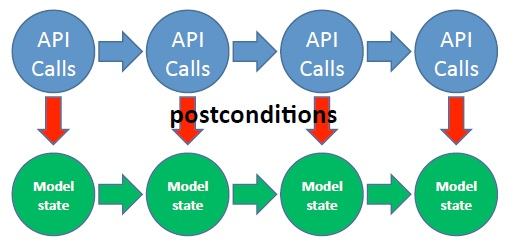
\includegraphics{pictures/api_calls.jpg}
\end{center}
\caption{Shows Erlang modeled states with calls against the C-code}
\label{FIG:api_calls}
\end{figure}
Early in the implementation phase Quickcheck found differences between the Erlang
and C-implementation. This was expected because every programmer makes mistakes.
The question was whether the fault was in the C-code or the Erlang code. Then
the API was thoroughly read and a conclusion was made. Either a bug in the
C-code was found or the Erlang-code needed to be corrected. There were however
cases when the API was ambiguous. In those cases the C-interpretation was chosen
as correct and the ambiguous specification written down.

Surprisingly bugs in the C-code was found early, even though it already run
sharp in lab environments; only a few specification requirements needed to be
implemented in Erlang.

If a bug in the C-code was discovered how should the work be continued? Since
Quickcheck terminates as soon as it finds a counter example something was needed to
be able to run further tests. Some alternatives were discussed.

\begin{enumerate}
        \item Fix the C-code, in other words change the C source code.
                \label{ENUMERATE:FixCCode}
        \item Mocking, in other words simulate different C-code output.
        \item Change the Erlang module to a faulty behavior to follow the C
                implementation.
\end{enumerate}

Item \ref{ENUMERATE:FixCCode} was chosen, see section \ref{sec:handlebugs}.

When thoroughly reading the AUTOSAR API not only ambiguous rules were found but
also rules that contradicted each other were recognized. In those cases the
implementation in the C-code was followed.

A great tool when a clear interpretation of the AUTOSAR specification was not
possible was to look into the C-code. Even though Quickcheck can be used to
test libraries when the actually source code is not available.

When the full module was implemented in Erlang code there had to be some assurance
for that every piece of code in the C implementation was actually tested.
Code coverage for the Erlang implementation was measured using the Erlang module
\emph{cover}. To be able to to measure the code coverage of the C-code the
commercial tool Bullseye Coverage was used. Only by using those tools it was
easy to see that the result was not good enough. The main problem seemed to be
that the WdgM was put in an absorbing state and after that following commands
did not test anything interesting. The reason for that an absorbing state was
reached was the availing of negative testing. The testing was negative because
invalid command sequences and arguments were generated.

Figure \ref{FIG:ONERUN} shows how the status of the watchdog manager changes
during the execution of API calls. After a number of commands the absorbing
state \emph{stopped} is reached.

\begin{figure}
  \begin{center}
    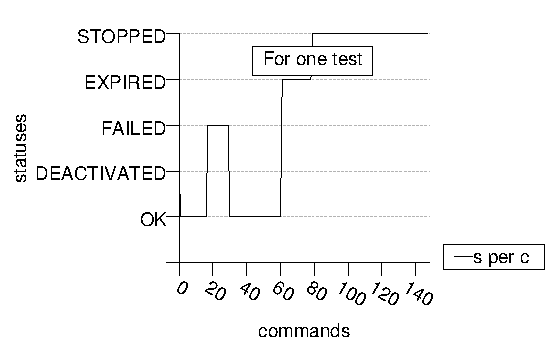
\includegraphics{generated_pictures/one_test_history_statuses_freescale.pdf}
    \caption{Shows how the status changes in the execution of one QuickCheck test}
    \label{FIG:ONERUN}
  \end{center}
\end{figure}

The next step was to tweak the generators, used by Quickcheck, to construct
valid API-calls. There were several branches in the C-code
that needed a specific sequence of API calls, with correct arguments, to be
reached. Also the tweaking of the generators could be implemented in a iterative
way. Change the probability properties of the generators and check the results.
The results were analyzed and the generators were tweaked even more to make the
results even better.

%% Just checking code coverage was however not good enough for our goals...

To get a better picture of the work flow used in this thesis see
figure \ref{fig:workflow}.

\begin{figure}[!ht]
\caption{Work flow}
\label{fig:workflow}
\fbox{
\parbox{\linewidth}{
\begin{enumerate}
\item Construct a model for an AUTOSAR module in Erlang
\item Run Quickcheck for this model and compare the results with the output from
the c code. \label{compare}
\item Tweak the generators for the test cases \label{generators}
    \item Evaluate the results
    \begin{enumerate}
      \item What is the state space?
      \item Which test cases are relevant?
      \item Collapse irrelevant states
      \item What can be said about the results?
    \end{enumerate}
\item Are the results good enough, does it satisfy the requirements for the ASIL
levels?
\item If not go the step \ref{compare}
\end{enumerate}
}}
\end{figure}
%even though correction of the C-code
%was not part of the thesis. Since there were actually code available, not
%only libraries, and most bugs was easy to fix this seemed like the best choice,
%see results.

A challenging step is the analysis of the results. If the testing tool returns zero
errors what does that say about the robustness of the input byte code? Passed
100 of 100 tests is just a statement and does not say anything more than that
some tests passed. Can tests be implemented in a clever way so that it is
possible to get some kind of confidence on the correctness of the code?

\section{Configurations}
When the code coverage was calculated it was recognized that every piece of code
wasn't executed. The reason seemed to be that the current configuration
disallowed the execution of some parts of the code, even though the
program behaved correctly. Because the implementation of the
Erlang module was independent of configurations it was easy to run
tests on several configuration which resulted in almost full coverage.

Three configurations with different complexity was used. The first
one, an example configuration (this will further on be called the
Example configuration), had many supervision functions configured in
each mode, and followed a strict execution of the program.

There were also a minimal configuration (BSI configuration) which, in
lack of supervision functions, only could change the global status
between \lstinline!WDGM_GLOBAL_STATUS_OK! and
\lstinline!WDGM_GLOBAL_STATUS_DEACTIVATED!. This on the other hand,
tested some null conditions, for example when there are no supervised
entities.

The last configuration, was one of the configurations that is used in
lab equipment and released to

The tweaking of generators, to achieve better test cases, seemed in some sense to be
configuration dependent. Better test cases were generated if the generators were
tweaked according to a specific configuration, see results.

\begin{figure}[!ht]
% Graphic for TeX using PGF
% Title: /home/oskar/documents/box.dia
% Creator: Dia v0.97.2
% CreationDate: Sat Sep  7 19:28:43 2013
% For: oskar
% \usepackage{tikz}
% The following commands are not supported in PSTricks at present
% We define them conditionally, so when they are implemented,
% this pgf file will use them.
\ifx\du\undefined
  \newlength{\du}
\fi
\setlength{\du}{15\unitlength}
\begin{tikzpicture}
\pgftransformxscale{1.000000}
\pgftransformyscale{-1.000000}
\definecolor{dialinecolor}{rgb}{0.000000, 0.000000, 0.000000}
\pgfsetstrokecolor{dialinecolor}
\definecolor{dialinecolor}{rgb}{1.000000, 1.000000, 1.000000}
\pgfsetfillcolor{dialinecolor}
\definecolor{dialinecolor}{rgb}{1.000000, 1.000000, 1.000000}
\pgfsetfillcolor{dialinecolor}
\fill (6.000000\du,7.000000\du)--(6.000000\du,11.000000\du)--(10.795000\du,11.000000\du)--(10.795000\du,7.000000\du)--cycle;
\pgfsetlinewidth{0.100000\du}
\pgfsetdash{}{0pt}
\pgfsetdash{}{0pt}
\pgfsetmiterjoin
\definecolor{dialinecolor}{rgb}{0.000000, 0.000000, 0.000000}
\pgfsetstrokecolor{dialinecolor}
\draw (6.000000\du,7.000000\du)--(6.000000\du,11.000000\du)--(10.795000\du,11.000000\du)--(10.795000\du,7.000000\du)--cycle;
% setfont left to latex
\definecolor{dialinecolor}{rgb}{0.000000, 0.000000, 0.000000}
\pgfsetstrokecolor{dialinecolor}
\node at (8.397500\du,9.195000\du){Testing Tool};
\pgfsetlinewidth{0.100000\du}
\pgfsetdash{}{0pt}
\pgfsetdash{}{0pt}
\pgfsetbuttcap
{
\definecolor{dialinecolor}{rgb}{0.000000, 0.000000, 0.000000}
\pgfsetfillcolor{dialinecolor}
% was here!!!
\pgfsetarrowsend{stealth}
\definecolor{dialinecolor}{rgb}{0.000000, 0.000000, 0.000000}
\pgfsetstrokecolor{dialinecolor}
\draw (10.795000\du,9.000000\du)--(12.000000\du,9.050000\du);
}
\pgfsetlinewidth{0.100000\du}
\pgfsetdash{}{0pt}
\pgfsetdash{}{0pt}
\pgfsetbuttcap
{
\definecolor{dialinecolor}{rgb}{0.000000, 0.000000, 0.000000}
\pgfsetfillcolor{dialinecolor}
% was here!!!
\pgfsetarrowsend{stealth}
\definecolor{dialinecolor}{rgb}{0.000000, 0.000000, 0.000000}
\pgfsetstrokecolor{dialinecolor}
\draw (0.000000\du,9.000000\du)--(6.000000\du,9.000000\du);
}
% setfont left to latex
\definecolor{dialinecolor}{rgb}{0.000000, 0.000000, 0.000000}
\pgfsetstrokecolor{dialinecolor}
\node[anchor=west] at (8.397500\du,9.000000\du){};
% setfont left to latex
\definecolor{dialinecolor}{rgb}{0.000000, 0.000000, 0.000000}
\pgfsetstrokecolor{dialinecolor}
\node[anchor=west] at (0.000000\du,10.000000\du){Module byte code};
% setfont left to latex
\definecolor{dialinecolor}{rgb}{0.000000, 0.000000, 0.000000}
\pgfsetstrokecolor{dialinecolor}
\node[anchor=west] at (3.000000\du,8.000000\du){};
% setfont left to latex
\definecolor{dialinecolor}{rgb}{0.000000, 0.000000, 0.000000}
\pgfsetstrokecolor{dialinecolor}
\node[anchor=west] at (2.000000\du,5.000000\du){Module specfication};
\definecolor{dialinecolor}{rgb}{1.000000, 1.000000, 1.000000}
\pgfsetfillcolor{dialinecolor}
\fill (12.000000\du,7.000000\du)--(12.000000\du,11.100000\du)--(17.800000\du,11.100000\du)--(17.800000\du,7.000000\du)--cycle;
\pgfsetlinewidth{0.100000\du}
\pgfsetdash{}{0pt}
\pgfsetdash{}{0pt}
\pgfsetmiterjoin
\definecolor{dialinecolor}{rgb}{0.000000, 0.000000, 0.000000}
\pgfsetstrokecolor{dialinecolor}
\draw (12.000000\du,7.000000\du)--(12.000000\du,11.100000\du)--(17.800000\du,11.100000\du)--(17.800000\du,7.000000\du)--cycle;
% setfont left to latex
\definecolor{dialinecolor}{rgb}{0.000000, 0.000000, 0.000000}
\pgfsetstrokecolor{dialinecolor}
\node at (14.900000\du,9.245000\du){};
\pgfsetlinewidth{0.100000\du}
\pgfsetdash{}{0pt}
\pgfsetdash{}{0pt}
\pgfsetmiterjoin
\pgfsetbuttcap
{
\definecolor{dialinecolor}{rgb}{0.000000, 0.000000, 0.000000}
\pgfsetfillcolor{dialinecolor}
% was here!!!
\pgfsetarrowsend{stealth}
{\pgfsetcornersarced{\pgfpoint{0.000000\du}{0.000000\du}}\definecolor{dialinecolor}{rgb}{0.000000, 0.000000, 0.000000}
\pgfsetstrokecolor{dialinecolor}
\draw (1.000000\du,5.000000\du)--(1.000000\du,6.000000\du)--(8.000000\du,6.000000\du)--(8.000000\du,7.000000\du);
}}
% setfont left to latex
\definecolor{dialinecolor}{rgb}{0.000000, 0.000000, 0.000000}
\pgfsetstrokecolor{dialinecolor}
\node at (14.900000\du,9.050000\du){Output};
% setfont left to latex
\definecolor{dialinecolor}{rgb}{0.000000, 0.000000, 0.000000}
\pgfsetstrokecolor{dialinecolor}
\node at (14.900000\du,9.850000\du){ analysis };
\end{tikzpicture}

\caption{Abstract implementation module}
\end{figure}

\section{Calling the API commands}
\label{SEC:CALLING_COMMANDS}
API calls were executed by QuickCheck using the \emph{run\_commands/1} function
according to \ref{SEC:QuickCheckIntro}. The runtime environment module (RTE) is
however responsible for the scheduling of the main function, which should be
executed in a given time interval. Since the RTE was not available when testing
the watchdog manager the main function was called randomly and it was
assumed that every time the main function was called a given amount of time had
passed.

Except the main function only one internal algorithm used by the watchdog
manager was time dependent, namely deadline supervision. A deadline supervision
consist of two checkpoints. One start checkpoint, one stop checkpoint and a
maximum time it shall take to reach the stop checkpoint after the start
checkpoint was reached. The AUTOSAR specification was however lacking of a
clear definition of how time should be represented. The C code just used ticks,
not actual time stamp, which was incremented every time the main function was
called. It was in other words assumed that the RTE was able to execute the main
function correctly and a fixed amount of ticks would always represent the same
amount of time. Accepting this solution it was easy to adopt the same approach
in the Erlang module. More about this can be found in section
\ref{SEC:FUNCTIONAL_SAFETY_TIME}.

\section{Model State}
The model state was constructed as easy as possible. Hence, even though it was
attempting to use a more efficient data structure, a simple record was used to
represent the model state. The main reason for that was to make it easier to
follow the model state when for instance using
\emph{eqc\_statem:show\_states/1}, see appendix \ref{APP:QUICKCHECK}. The
efficiency of the test model was considered less relevant then the readability
of the model state.  The idea was to make it easy to find the actual bug, when
there were conflicts between the C-code and the Erlang module, and running the
actual tests was not considered time or memory critical.


\chapter{Result}
\label{CHAPTER:RESULTS}
%TODO Why is the global status relevant
%Is there other things that should be described in the report

\section{State Machine}
The watchdog manager has a state machine, shown in
figure~\ref{FIG:GLOBALSTATUSES}. Its transitions depend on the changes of the
global variables, and the current state. If the behavior of the watchdog manager
is correct and the manager is activated, it will stay in the state
'WDGM\_GLOBAL\_STATUS\_OK'. There are however lots of reasons for that the
status will change from the correct state. It depends on the arguments of the
API calls but also the order of the commands that are called and which AUTOSAR
configuration that is supplied. The configuration is important because it
specifies the tolerance of faulty behavior the watchdog should have. It could
also indirectly disable some states and state transition or make some transition
more likely to happen. The effect can for instance come from the number of
checkpoints supplied in the configuration. A correct behavior of the watchdog
manager depends on that checkpoints are reached and does so in the right order
and right timing.

Besides the transition between the deactivated and the OK states, the only
function that can give rise to state transitions for the global status, is the
main function. In an working ECU, the main function should continuously be
called, in a configured time interval, by the run time environment (RTE). Note
that the timing is not used when using QuickCheck, see section
\ref{SEC:CALLING_COMMANDS}.

\begin{figure}[h!]
  \begin{center}
    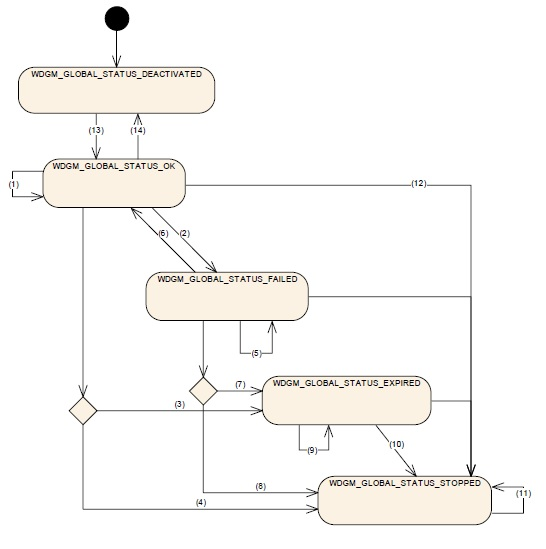
\includegraphics{pictures/globalstatuses.jpg}
  \end{center}
  \caption{State diagram that shows possible trasitions between states}
  \label{FIG:GLOBALSTATUSES}
\end{figure}

\section{Configurations}
The WdgM was tested using three different configurations. The configurations
were of different complexity. One was a minimal configuration, one a example
configuration and one was a live configuration, used in actual implementations.

Because there is only a small number of commands that influences the state
transitions, those commands were tweaked and therefore was generated more
often. On the other hand, all get-functions were tweaked to not be generated as often.

\subsection{BSI}
A highly simplified configuration, \emph{BSI}, gives in some sense good results.
Using this configuration the WdgM was never hitting the absorbing state
according to figure \ref{FIG:GLOBALSTATUSES}.  However looking at the state
transitions, comparing figure \ref{FIG:GLOBALSTATUSES} and table
\ref{TABLE:STATUSES_BSI}, only two states are hit. This happens
because the configuration is to simple, it is actually impossible to hit
any other states then \emph{'GLOBAL\_STATUS\_OK'} or
\emph{'GLOBAL\_STATUS\_DEACTIVATED'}. There are no checkpoints or supervision
functions configured for the \emph{BSI} configuration.
It is easy to run tests using this configuration but it does not, by it self,
fully test the code because some specification requirements will never be
tested. The untested requirements are mainly requirements for supervision
functions that are, according to the configuration, never supposed to be
run. Those untested requirements leaves also other requirements untested because
the watchdog manager never reaches a state when those other requirements must
hold.

Figure~\ref{FIG:COMMANDS_BSI} shows how many times a certain command was
generated versus the length of the command sequence that was generated. E.g. the
function \lstinline!WdgM_CheckpointReached! had in average a little more than
40\% of all calls. This is because, in any other configuration, the supervision
functions demand that a certain number of checkpoints is reached before the next
main function is called \footnote{This is however not completely true, but it
  gives the general idea.}. There is also a dependency the other way around. The
main function has to be called a certain number of times before
\lstinline!WdgM_CheckpointReached! is called on a certain supervised
entity. This is why that function also has quite high proportions. Other
functions that stands out is \lstinline!WdgM_SetMode! and \lstinline!WdgM_Init!.
\lstinline!WdgM_Setmode! is called because different modes can have different
supervision functions and supervised entities. That is why we need to call this
function often. It should retain the states of supervised entities that is
activated in the new mode and should reset the local state if the entity is
deactivated in the new mode. The function \lstinline!WdgM_Init! is in contrast
called lesser and lesser times. This function is only needed when the global
state is deactivated. It has more likelihood to be generated among the first
commands in the command sequence, or right after a \lstinline!WdgM_DeInit!.

\begin{figure}[h!]
  \begin{center}
    \subfigure[Shows percentage of each possible command executed]{
      \label{FIG:COMMANDS_BSI}
      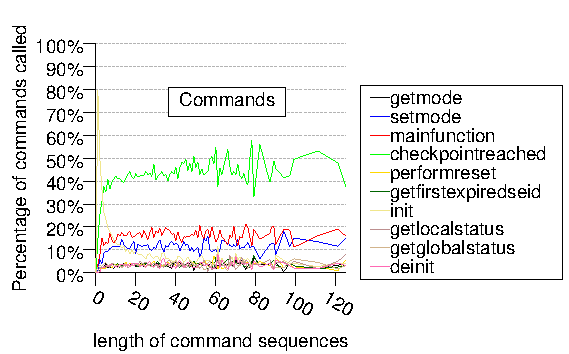
\includegraphics{generated_pictures/history_commands_bsi.pdf}
    }

    \subfigure[Shows percentage of each possible global status hit]{
      \label{FIG:STATUSES_BSI}
      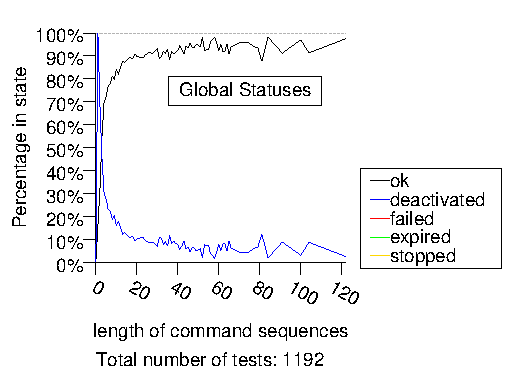
\includegraphics{generated_pictures/history_statuses_bsi.pdf}
    }
  \end{center}
  \caption{BSI configuration}
  \label{FIG:BSI}
\end{figure}

\begin{table}[h!]
  \caption{bsi configuration}
  \label{TABLE:STATUSES_BSI}
  
    \begin{tabular}{r|ccccc}
        \hline
        \multicolumn{6}{c}{Number of tests: 2850} \\
        \hline
        \backslashbox{From}{To}
                    & DEACTIVATED & EXPIRED & FAILED & OK & STOPPED \\
        \hline
        DEACTIVATED & \bf{02.23}\% & 00.00\%       & 00.00\%       & \bf{09.12}\% & 00.00\% \\
        EXPIRED     & 00.00\%       & \bf{00.00}\% & 00.00\%       & 00.00\%       & \bf{00.00}\% \\
        FAILED      & 00.00\%       & \bf{00.00}\% & \bf{00.00}\% & \bf{00.00}\% & \bf{00.00}\% \\
        OK          & \bf{03.24}\% & \bf{00.00}\% & \bf{00.00}\% & \bf{85.41}\% & \bf{00.00}\% \\
        STOPPED     & 00.00\%       & 00.00\%       & 00.00\%       & 00.00\%       & \bf{00.00}\%
      \end{tabular}
    

\end{table}

\subsection{freescale}
The freescale configuration is, compared to BSI, a more realistic configuration.
All supervision algorithms are configured and there are both external and
internal graphs for logical supervision. It is also the configuration, mainly
used at Mecel. The state machine for the global status is totally covered by
running QuickCheck, see table \ref{TABLE:STATUSES_FREESCALE} and figure
\ref{FIG:GLOBALSTATUSES}.


\begin{figure}[h!]
  \begin{center}
    \subfigure[Shows percentage of each possible command executed]{
      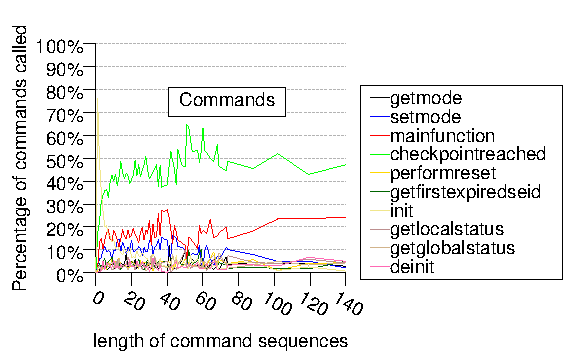
\includegraphics{generated_pictures/history_commands_freescale.pdf}
      \label{FIG:COMMANDS_FREESCALE}
    }
    \subfigure[Shows percentage of each possible global status hit]{
      \label{FIG:STATUSES_FREESCALE}
      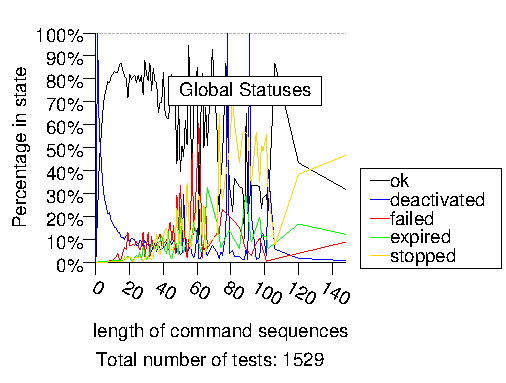
\includegraphics{generated_pictures/history_statuses_freescale.pdf}
    }
  \end{center}
  \caption{Freescale configuration}
  \label{FIG:FREESCALE}
\end{figure}

\begin{table}[!h]
  \caption{Freescale configuration}
  \label{TABLE:STATUSES_FREESCALE}
  
    \begin{tabular}{r|ccccc}
        \hline
        \multicolumn{6}{c}{Number of tests: 1023} \\
        \hline
        \backslashbox{From}{To}
                    & DEACTIVATED & EXPIRED & FAILED & OK & STOPPED \\
        \hline
        DEACTIVATED & \bf{02.43}\% & 00.00\%       & 00.00\%       & \bf{08.32}\% & 00.00\% \\
        EXPIRED     & 00.00\%       & \bf{03.36}\% & 00.00\%       & 00.00\%       & \bf{00.11}\% \\
        FAILED      & 00.00\%       & \bf{00.17}\% & \bf{07.77}\% & \bf{00.12}\% & \bf{00.11}\% \\
        OK          & \bf{02.56}\% & \bf{00.18}\% & \bf{00.87}\% & \bf{69.53}\% & \bf{00.12}\% \\
        STOPPED     & 00.00\%       & 00.00\%       & 00.00\%       & 00.00\%       & \bf{04.34}\%
      \end{tabular}
    

\end{table}

\subsection{example}

\begin{figure}[h!]
  \begin{center}
    \subfigure[Shows percentage of each possible command executed]{
      \label{FIG:COMMANDS_EXAMPLE}
      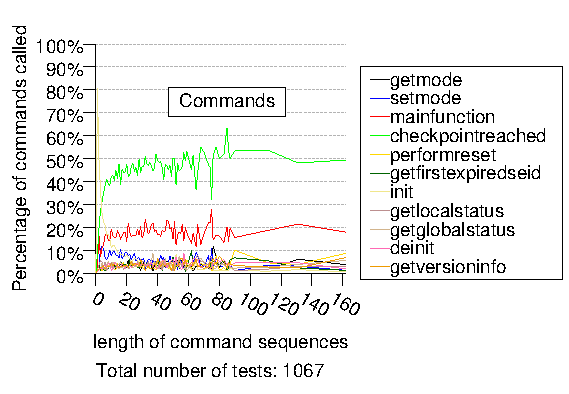
\includegraphics{generated_pictures/history_commands_example.pdf}
    }

    \subfigure[Shows percentage of each possible global status hit]{
      \label{FIG:STATUSES_EXAMPLE}
      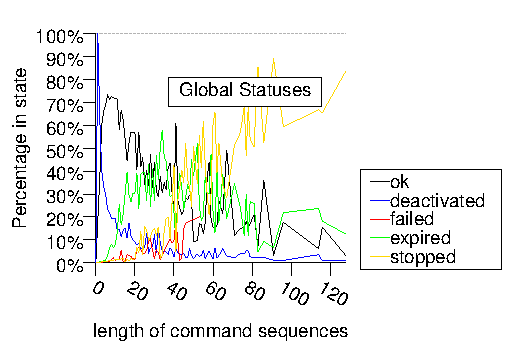
\includegraphics{generated_pictures/history_statuses_example.pdf}
    }
  \end{center}
  \caption{Example configuration}
  \label{FIG:EXAMPLE}
\end{figure}

\begin{table}[!h]
  \caption{example configuration}
  \label{TABLE:STATUSES_EXAMPLE}
  
    \begin{tabular}{r|ccccc}
        \hline
        \multicolumn{6}{c}{Number of tests: 3877} \\
        \hline
        \backslashbox{From}{To}
                    & DEACTIVATED & EXPIRED & FAILED & OK & STOPPED \\
        \hline
        DEACTIVATED & \bf{02.59}\% & 00.00\%       & 00.00\%       & \bf{07.81}\% & 00.00\% \\
        EXPIRED     & 00.00\%       & \bf{24.77}\% & 00.00\%       & 00.00\%       & \bf{00.81}\% \\
        FAILED      & 00.00\%       & \bf{00.12}\% & \bf{02.87}\% & \bf{00.00}\% & \bf{00.04}\% \\
        OK          & \bf{01.68}\% & \bf{02.50}\% & \bf{00.39}\% & \bf{40.22}\% & \bf{00.14}\% \\
        STOPPED     & 00.00\%       & 00.00\%       & 00.00\%       & 00.00\%       & \bf{16.07}\%
      \end{tabular}
    

\end{table}

\section{Handle bugs in the C code}
\label{sec:handlebugs}

\section{Functional safety analysis}
\subsection{Definition of time}
\label{SEC:FUNCTIONAL_SAFETY_TIME}

\section{Statistics}

\section{Functional safety analysis}
Since one important part of the functional safety concept is that it must be
taken in consideration during the hole development process, one can not simply
say that QuickCheck makes it possible to acquire functional safety. There must
first be a number of assumptions. Not even if it is assumed that
every step in the development, until the actual implementation of the watchdog
manager, satisfies the requirements one also has to assume that the remaining
part of the development, towards a finished vehicle, follows the same
constrains. Even further, if this is assumed, there is one important
assumption left before
one can even reason about how QuickCheck can benefit.
This assumptions lies in that the model for the watchdog
manager is correct, namely the AUTOSAR specification.


\chapter{Discussion}

The model has been implemented in an iterative way. Function for
function, requirement for requirement. This process is very easy with
the use of QuickCheck.  In the beginning there were alot of negative
testing, because we didn't care about tweaking the generators.
By limiting the state space for negative tests, we achieved a better
ratio for positive testing when generating random tests. This was done
by letting some command sequences weight more than others when
QuickCheck generates the test cases. In
figure~\ref{QUICKCHECK:TWEAKING} we show how the state space is
minimized when QuickCheck has been tweaked.

\begin{figure}[!ht]
  \begin{center}
    \begin{minipage}[b]{0.6\linewidth}
      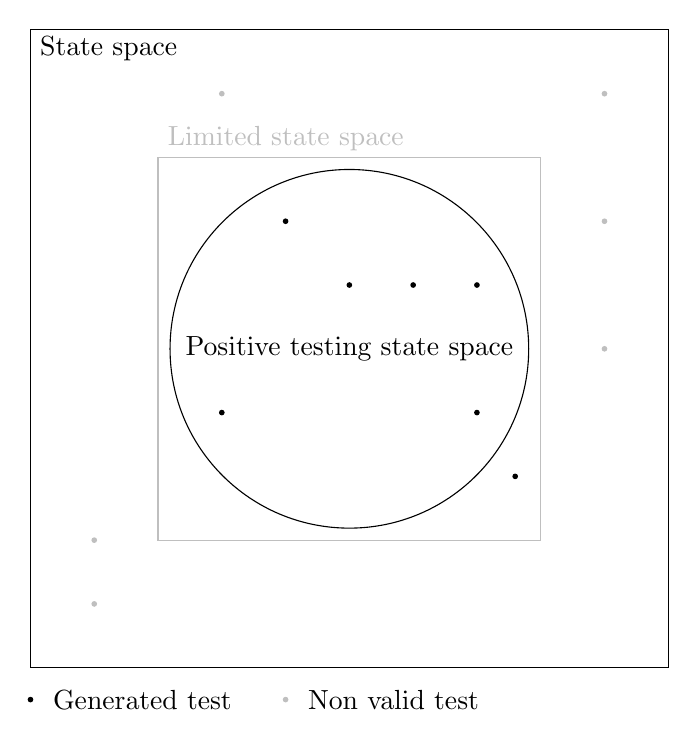
\begin{tikzpicture}[scale=0.81,
  valid/.style={fill=black},
  unvalid/.style={fill=black!25, color=black!25}]
\draw (0,0) rectangle (10,10) node [below, right] at
(0,9.7) {State space};
\draw [color=black!25] (2,2) rectangle (8,8) node [above, right] at
(2,8.3) {Limited state space};
\draw (5, 5) circle (80pt) node at (5,5) {Positive testing state space};

\draw [unvalid] (1,1) circle (1pt);
\draw [unvalid] (1,2) circle (1pt);
\draw [valid] (3,4) circle (1pt);
\draw [unvalid] (3,9) circle (1pt);
\draw [unvalid] (9,5) circle (1pt);
\draw [unvalid] (9,9) circle (1pt);
\draw [valid] (7,6) circle (1pt);
\draw [unvalid] (9,7) circle (1pt);
\draw [valid] (5,6) circle (1pt);
\draw [valid] (4,7) circle (1pt);
\draw [valid] (6,6) circle (1pt);
\draw [valid] (7,4) circle (1pt);
\draw [valid] (7.6,3) circle (1pt);

\draw [valid] (0,-0.5) circle (1pt) node [right] at (0.2,-0.5)
{Generated test};
\draw [unvalid] (4,-0.5) circle (1pt) node [right, color=black] at (4.2,-0.5)
{Non valid test};
\end{tikzpicture}
    \end{minipage}
  \end{center}
  \caption{The state space when tweaking QuickCheck's generators.}
  \label{QUICKCHECK:TWEAKING}
\end{figure}
The outer box in figure~\ref{QUICKCHECK:TWEAKING} represents the full
state space, and the inner circle represents positive test cases. This
means that all test cases outside of the circle represents negative
test cases. When tweaking generators it mean we can limit some of the
negative test state space, in order to have QuickCheck generate more
interesting positive test cases. The black dots in the figure
represents different generated test cases, and the gray dots
represents test cases which will not be generated after the new
limitations.

As an example, it is unnecessary to test functions if the watchdog
manager state machine has not been initialized with a call to the
\lstinline!WdgM_Init! function. We can weight the generation
of the \lstinline!WdgM_Init! function to be called with a higher ratio
if the state machine is not initialized yet.

\begin{lstlisting}[style=erlang, literate={_}{\_}1]
weight(S,  'WdgM_Init') ->
  case S#state.initialized of
    true                           -> 1;
    _                              -> 200
  end;
\end{lstlisting}

Sometimes the model needs to be corrected because of ambiguities in
AUTOSAR or errors in the model. Quite often it was the C-code that had
the errors and needed to be corrected.  Easier when you do white box
testing, when the source code is known, because then you can really
check the code and compare with the requirements.

The C-code coverage was measured differently from the Erlang code
coverage, which used line coverage instead of condition/decision
coverage. Recursion is often used in functional programming languages
as Erlang, therefore it is not as suited for condition/decision
coverage as C-code is. Erlang also comes with a coverage library,
which makes it easy to use. On the other hand, measuring line coverage
in a imperative language like C is a bit redundant since statements
are executed sequentially. Therefore conditions/decision coverage
seems more reasonable.

We achieved fair coverage of the C-code, around 85\%, and the Erlang
code, around 97\%. The problem was the requirements, where we achieved
around 50\%. It would help if a QuickCheck model was implemented for
the whole system as well. Many of the requirements had dependencies in
other modules, and some requirements for the file structure, the
configuration or even the generation of files.

QuickCheck is good for overall testing, and can help with raising the
functional safety of modules.

%% analys av resultat
%% - coverage på modell och c-kod genom cover (erlang) och bullseye (c-kod)
%% - statistik på quickcheck körningar.

Stripped of comments and blank lines, the implemented Erlang model is
almost 1300 lines of code. This is to be compared with the C-code
which is over 14500 lines of code.
%% cat src/* inc/* generated_cfg/*.[c,h] stub/* rte/* gcc/* | grep -vP
%% ^[[:space:]]?'/\*' | grep -vP ^[[:space:]]?'\*' | grep -vP
%% ^[[:space:]]?'\\\*' | grep -v ^[[:space:]]$ | wc -l


\section{Future work}
Some interesting thing we wanted to do from the beginning was to implementing
another module, preferably one that has some kind of dependency with the
watchdog manager. This is because then, it would be possible to testing towards
the phase ``system integration and testing'' in ISO~26262 and get even better
results.

Another good idea is to do more negative testing, and testing of null
pointers. This should be done to raise the coverage for the C-code to even
better levels.

We could also try new configurations. More configurations = better testing.

\chapter{Conclusion}
It is possible to achieve some functional safety using QuickCheck, at
least within the software units. There are however a number of
ISO~26262 requirements that is not possible to achieve with only a
software testing tool. For example requirements that verifies the
hardware specifications or how the safety plan should be made. It is
hard to use the ISO~26262 V reference model if the software units do
not follow system properties that has been verified by a system
model. Because AUTOSAR is written with informal syntax, it can't be
used to verify the software units. This means one must translate the
AUTOSAR requirements to formal syntax and verify that the formal
requirements means the same as the informal requirements.

It is important to not only measure the state space, but also the code
coverage. This can also be done with the use of QuickCheck. It is easy
to measure Erlang coverages, and it is also easy to specify which
compiler QuickCheck should use to perform C code coverages.
QuickCheck gathers information about the state space, which is
outputted after a test has been run.

Both negative and positive testing can be implemented with the use of
QuickCheck. Negative testing can be time-consuming because the program
quickly comes to an absorbing state. It is therefor important to tweak
the generators correctly.

Integration tests can also easily be implemented, by connecting
several AUTOSAR modules. When doing this even more ISO~26262
requirements can be evaluated and verified.

One needs to be aware of the configuration of the AUTOSAR module which
is going to be implemented, because it may contain variables that is
not safe to turn off. It may also be difficult to reach the whole
state space if the configuration is to simple or to complex.

\bibliographystyle{vancouver}
\bibliography{references}

\appendix
\chapter{Introductions to QuickCheck}
\label{APP:QUICKCHECK}
\lstset{style=erlang}
\label{SEC:QuickCheckIntro}

\section{The General Idea}
The general idea with QuickCheck, is here explained by using an example.
Let us say that one has a \emph{sort} function that takes a list $Xs$ of any
sortable items and returns the sorted version $Ys$ of $Xs$. To verify the
correctness of this function it is possible to look at certain properties
that must hold for a correctly implemented sort function. For instance:

\noindent The arity of $Y$ must be the same.
\begin{equation}
        |Xs| = |Ys|
\end{equation}

\noindent The elements of $Ys$ must actually be sorted.
\begin{equation}
    y_{i-1} \leq y_i, \forall y_i \in Ys, i \neq 0
\end{equation}

\noindent For all permutations $Pe(Xs)$ holds:
\begin{equation}
sort(Zs) = Ys, \forall Zs \in Pe(Xs)
\end{equation}

\noindent The sets $Xs$ and $Ys$ contain the same elements.
\begin{equation}
        x \in Xs \leftrightarrow x \in Ys
\end{equation}
Instead of specifying own test cases QuickCheck makes it possible to write such
properties, automatically generates test cases and checks that the properties
specified actually holds.

\section{Testing C-code}
QuickCheck is a testing tool for the programming language Erlang, but it is
possible to efficiently test C-code, using QuickCheck, by performing API-calls
against the C-code within Erlang.  Lets say that there is a \emph{Queue}
implementation in C that has a function for creating a new queue as well
as functions for inserting and retrieving elements from a queue structure.

\begin{lstlisting}[style=c]
typedef struct
{
   int size;
   int head;
   int tail;
   int* buffer;
} Queue;

Queue* new(int size) { ... }
int put(Queue* q, int element) { ... }
int get(Queue* q) { ... }
\end{lstlisting}
This program has a number of properties that should hold. For
instance:
\begin{itemize}
\item When creating a new queue, the C function should return an
address to the memory where it have allocated space.
\item The function \emph{put} should insert the element into the queue
and return the element.
\item It should be possible to dequeue an element in the order it was
inserted with the function \emph{get}.
\end{itemize}
Such properties can be used when using QuickCheck.
%Instead of specifying own test cases QuickCheck makes it possible to
%write such properties, automatically generates test cases and checks
%that the properties specified actually holds.

When testing C code with QuickCheck one uses state based
testing. Which means that a model state $S$ is passed around and
checked against API calls according to figure \ref{FIG:API_CALLS}.

\begin{figure}[!h]
  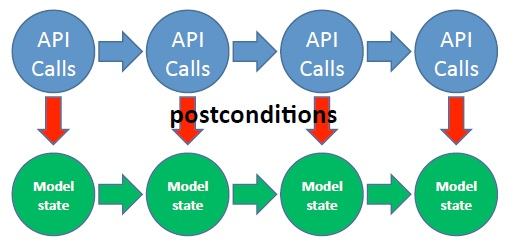
\includegraphics{pictures/api_calls.jpg}
  \caption{Shows state based testing against API and model state}
  \label{FIG:API_CALLS}
\end{figure}
First a model of the queue must be implemented in Erlang code.
It is also needed to implement a representation of the current state of the queue.

\begin{lstlisting}
-record(state, {ptr, queue}).

new_next(_S, Pointer, _) ->
   #state{ptr=Pointer, queue=[]}.
put_next(S, _, [_, X]) ->
   S#state{queue = S#state.queue++[X]}.
get_next(S, _, _) ->
   S#state{queue = tl(S#state.queue)}.
\end{lstlisting}

The \emph{record} will contain information needed to successfully
test the states of the program. It has two variables;
\emph{ptr} which is the pointer to the queue and
\emph{queue} which is a list defining all inserted elements in the queue.

QuickCheck must also be told how to call the C-functions.
\begin{lstlisting}
new(Size) ->
  q:new(Size).
put(Ptr, Val) ->
  q:put(Ptr, Val).
get(Ptr) ->
  q:get(Ptr).
\end{lstlisting}

Now the postconditions, program properties that must hold, are defined.
\begin{lstlisting}
new_post(_S, _Arguments, ReturnValue) ->
  case ReturnValue of
    {ptr, "Queue", _} -> true;
    _                 -> false
  end.
put_post(_S, [_, InsertedValue], ReturnValue) ->
  ReturnValue == InsertedValue.
get_post(S, _Arguments, ReturnValue) ->
  ReturnValue == hd(S#state.elements).
\end{lstlisting}

To be able to test these properties QuickCheck needs to know how to generate
arguments for every functions.
\begin{lstlisting}
new_args(_S) ->
   [nat()].
put_args(S) ->
   [S#state.ptr, int()].
get_args(S) ->
   [S#state.ptr].
\end{lstlisting}
The functions \emph{nat()} and \emph{int()} are generators
defined by QuickCheck to generate arbitrary natural numbers and integers.

To test the functions \emph{put}, \emph{get} and \emph{new} defined in the C-code a QuickCheck
property is written in the following way.  \lstset{style=erlang}
\begin{lstlisting}
prop() ->
  ?FORALL(Cmds, commands(),
          begin
            ... = run_commands(Cmds)
          end).
\end{lstlisting}

The function \emph{commands()} is a generator that looks
for functions defining the API-calls, such as \emph{new}, \emph{put} and
\emph{get}, in the Erlang module. The \emph{commands()} function then combines
every function $api_i$ defining an API-call with a function $arg_i$ which
generates the arguments to $api_i$.

After the property has been implemented, it can be tested by:

\begin{lstlisting}
eqc:quickcheck(prop()).
\end{lstlisting}

It is possible define how many tests QuickCheck should execute and also if the
states of the model should be shown:
\begin{lstlisting}
eqc:quickcheck(eqc:numtests(N, eqc_statem:show_states(prop()))).
\end{lstlisting}

\section{QuickCheck Modules}
QuickCheck consist of several Erlang modules.
%%eqc
\subsection{eqc}
The module \emph{eqc} is the main QuickCheck module. This module defines a lot
of macros that can be used when writing properties and also basic functions
like \emph{quickcheck}.

\subsection{eqc\_gen} The module is used for generations of test cases. The module
contains various functions and macros for this purpose. There are some
predefined generators, for instance for integers and characters etcetera, but it
is quite easy to construct a generator for almost any data type. Just to get the
idea follows code for a string generator.
\begin{lstlisting}
    ?LET(Pat, nat(), vector(Pat, char()))
\end{lstlisting}
The macro \emph{?LET} binds a generated value from the second argument, to \emph{Pat} which can be
used in the third argument. The above code binds a natural number, from the
generator \emph{nat()}, to \emph{Pat} and creates a vector with length
\emph{Pat} of characters.

A generator can also be weighted, or in other words certain values can be more
likely to be generated than others.

\begin{lstlisting}
?LET(Pat, nat(), vector(Pat,
                        frequency([{1, choose(0,127)},
                                   {3, 32}])))
\end{lstlisting}
The code above will also generate a string of length \emph{Pat}, but the
generation of the white space character will be 3 times more likely to happen
than a uniformly random character.

%%% eqc_c
\subsection{eqc\_c} Contains the C-testing interface. In other words how to
communicate with C-code.

\begin{lstlisting}
eqc_c:start(q, [{c_src, "q_api.h"},
                {additional_files, ["queue.o"]}])
\end{lstlisting}
The code above starts the C-program \emph{queue.o}, and an Erlang module is
created with the name of the first parameter, \emph{q}. This module can now
be used within Erlang to call the C-program.

%%% eqc_statem
\subsection{eqc\_statem}
\label{SEC:EQC_STATEM}
Offers state based testing as shown above. A command has a definition, precondition,
postcondition, and a next function.

Noticeable is that only the post function may depend on the
C-code. QuickCheck has a generation step where tests are generated
according to the precondition and the model state. The C-code is run
first after the generation step and can only be used to check
postconditions. This is actually what one want because it would be
pointless to execute a program and then test it depending on the
execution of the same program and not the model itself. For instance
if we let the next state function depend on the C-program, then the
model will be faulty if the C-program has incorrect behavior.

Possible preconditions for queue example above could be that the
functions \emph{put} and \emph{get} can only be called if
the queue has first been created and \emph{new} can only be
called with a size greater than zero.
\begin{lstlisting}
new_pre(_S, [Size]) ->
  Size > 0.
put_pre(S) ->
  (S#state.ptr /= undefined) andalso
  (length(S#state.queue) < S#state.size).
get_pre(S) ->
  (S#state.ptr /= undefined) andalso
  (length(S#state.queue) > 0).
\end{lstlisting}

%car_xml
\subsection{car\_xml}
Additional to the commercial version, there is a \emph{car} module. This module is
specifically created to parse AUTOSAR XML configuration files.

%% relevans?
\subsection{Other modules}
\label{APP:SEC:OTHERMODULES}
There are also other modules; for instance a module for mocking C-code. Or in
other words, if one has a C-function that is declared but the
definition is missing, one can simulate its output. This is
however not used in this thesis.

%%%%%%%%%%%%%%%%%%%%%%%%%%%%%%%%%%%%%%%%%%%%%%%%%%%%%%%%%%%%%%%%%%%%%%%%%%%%%%%%

\lstset{style=autosar}
\chapter{The Watchdog Manager (WdgM)}
\label{APPENDIX:WDGM}
The watchdog is a basic AUTOSAR module. It's purpose is to supervise a programs
execution by triggering hardware watchdogs entities. For the hole description of
the module see the AUTOSAR specification.

\section{Supervision, Checkpoints and Graphs}
The watchdog supervises the execution of so called \emph{Supervised Entities}.
Important places in a supervised entity are marked as checkpoints. There are at
least one checkpoint for every supervised entity. The checkpoints and
transitions between checkpoints are defined as graphs. Checkpoints and
transitions between checkpoints within a given supervised entity are marked as
internal graphs. There may however be transitions between checkpoints of
different supervised entities, such graphs are marked as external graphs.
Available graphs are supplied by the configuration. There may be different
graphs for different modes of the watchdog manager.
%Lite matematiska utryck kanske?

There are three supervision algorithms to verify the correctness of supervised
entities.
\begin{itemize}
\item Logical Supervision: \\
Logical supervision verifies if graphs are executed in the correct order. \\ Let
$G = (V,E)$ be a internal graph for a supervised entity $S$ such that $\forall c_k
\in V \rightarrow c_i \in S$. For the graph $G$ there exist a start checkpoint
$c_s \in V$ and a final checkpoint $c_f \in V$. The logical supervision
checks that the first checkpoint $c_1$ that is reached has the property $c_1 =
c_s$ and for every reached checkpoint $c_j$ there exists an edge
$(c_{j-1},c_{j}) \in E, j \neq 1$.
\item Alive Supervision: \\
  Alive supervision periodically verifies the timing of transitions and
checkpoints reached in a graph.
\item Deadline Supervision: \\
  Deadline supervision does the same as alive supervision but aperiodically.
\end{itemize}

\section{Global Status}
\label{APP:GLOBALSTATUS}
The global status represents the current state of the whole watchdog
manager. There are five different statuses.
\begin{itemize}
\item WDGM\_GLOBAL\_STATUS\_DEACTIVATED \\
  The watchdog manager is in a resting state, deactivated, and will not execute
  any supervision functions.
\item WDGM\_GLOBAL\_STATUS\_OK \\
  The watchdog manager is in a correct state.
\item WDGM\_GLOBAL\_STATUS\_FAILED \\
  A failure has occurred for an alive supervision and the watchdog is configured
  to have a tolerance against this kind of error.
\item WDGM\_GLOBAL\_STATUS\_EXPIRED \\
  A fault has happened and the watchdog is configured to postpone the error
  reaction. In contradiction to
  \emph{WDGM\_GLOBAL\_STATUS\_FAILED} there is no recovery mechanism for this
  state and the watchdog manager will eventually reach the state
  \emph{WDGM\_GLOBAL\_STATUS\_STOPPED}.
\item WDGM\_GLOBAL\_STATUS\_STOPPED \\
  This is an absorbing state of the watchdog state machine. Recovery mechanisms
  will be started and usually a watchdog reset will occur.
\end{itemize}
The different statuses are related to each other according to figure~\ref{APP:FIG:GLOBALSTATUS}.
There is only a small number of functions that is allowed to change the global
status; those are the main function, the initialization function and the
de-initialization function. The main function decides the next global status by
checking the local statuses of the supervised entities and the current global
status. The initialization function should only be able to change the global
status from deactivated to ok, and the de-initialization function from ok to deactivated.

\begin{figure}[!ht]
  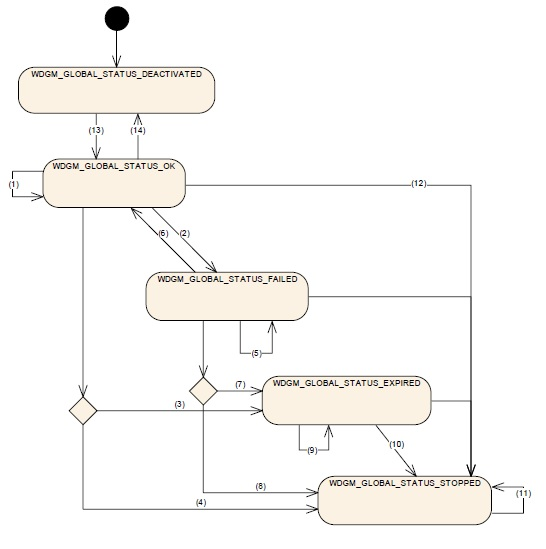
\includegraphics{pictures/globalstatuses}
  \label{APP:FIG:GLOBALSTATUS}
  \caption{The possible global statuses represented as a graph}
\end{figure}

\section{Local Status}
A local status is a status of one supervised entity and could be set according
to the current local status and the results of the supervision functions. There
are four different local statuses. Init setmode mainfunction

\begin{itemize}
  \item WDGM\_LOCAL\_STATUS\_DEACTIVATED\\
    If a supervised entity is set to deactivated, it will not be checked by the
    supervision functions.
  \item WDGM\_LOCAL\_STATUS\_OK\\
    The supervised entity is in a correct state.
  \item WDGM\_LOCAL\_STATUS\_FAILED\\
    Alive supervision for the supervised function has failed.
  \item WDGM\_LOCAL\_STATUS\_EXPIRED\\
    A fault has been observed within the supervised function. The main function
    will save the identification of the first supervised entity which reaches this
    state.
\end{itemize}
Figure \ref{APP:FIG:LOCALSTATUSES} describes the state machine for the local
status of a supervised entity.

\begin{figure}[!ht]
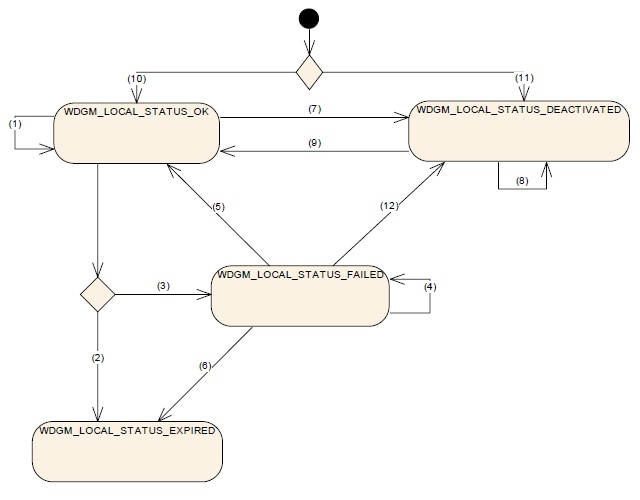
\includegraphics{pictures/localstatuses}
\label{APP:FIG:LOCALSTATUSES}
\caption{The possible local statuses represented as a graph}
\end{figure}

\section{API functions}
\label{APP:API_CALLS}
\subsection{WdgM\_Init}
Initializes the watchdog manager by setting, among other things, the local
status of all supervised entities to either WDGM\_LOCAL\_STATUS\_OK or
WDGM\_LOCAL\_STATUS\_DEACTIVATED. It also changes the global status to
WDGM\_GLOBAL\_STATUS\_OK.
\subsection{WdgM\_DeInit}
Deinitializes the watchdog manger.
\subsection{WdgM\_GetVersionInfo}
Returns the version info of the watchdog manager module.\footnote{The function shall not change the
internal state of the watchdog manager and should be side effect free.}
\subsection{WdgM\_SetMode}
Sets a new mode for the watchdog manager.
\subsection{WdgM\_GetMode}
Returns the current mode for the watchdog manager\footnotemark[\thefootnote].
\subsection{WdgM\_CheckpointReached}
\label{SEC:CHECKPOINTREACHED}
Performs deadline and logical supervision for a given supervised entity.
\subsection{WdgM\_GetLocalStatus}
Returns the local status of a supervised entity\footnotemark[\thefootnote].
\subsection{WdgM\_GetGlobalStatus}
Return the global status of the watchdog manager\footnotemark[\thefootnote].
\subsection{WdgM\_PerformReset}
Shall set the trigger condition for all configured watchdogs to zero and
thereby causing the hardware watchdogs to cause an external hardware reset.
\subsection{WdgM\_GetFirstExpiredSEID.}
Returns the supervised entity that first reached the state
\emph{WDGM\_LOCAL\_STATUS\_EXPIRED}\footnotemark[\thefootnote].
\subsection{WdgM\_MainFunction}
\label{SEC:MAINFUNCTION}
The main function is periodically called, it first updates the local statuses by
running alive supervision for the supervised entities and then sets the global
status depending on the current state of the watchdog manager; this includes the
new values of the local statuses.

%%%%%%%%%%%%%%%%%%%%%%%%%%%%%%%%%%%%%%%%%%%%%%%%%%%%%%%%%%%%%%%%%%%%%%%%%%%%%%%%

\setlength{\parindent}{0pt}
\begin{comment}
\chapter{Bugs in C-code}
\section{Failed reference supervision cycles is changed to early}
When applying the requirements [WDGM203], [WDGM204], [WDGM300], [WDGM205], the counter for failed reference cycles has already been
changed. The old value for the counter is needed.

\subsection{Severity}
Significant

\subsection{Steps to reproduce}
\begin{lstlisting}
WdgM_Init(Configuration)
WdgM_SetMode(0, 1)
WdgM_MainFunction()
WdgM_MainFunction()
WdgM_MainFunction()
WdgM_MainFunction()
WdgM_MainFunction()
\end{lstlisting}
\paragraph{Expected results:}
The global status should be \lstinline!WDGM_GLOBAL_STATUS_EXPIRED!.
\paragraph{Actual results:}
The global status is set to \lstinline!WDGM_GLOBAL_STATUS_FAILED!.

\subsection{Further comments}
There is possibly some additional unwanted behavior because of this,
that one should be aware of.

Because of the alive supervision results does not change appropriately
with the local status of the supervised entity, there is a possibility
where you don't reach the requirements [WDGM300] or [WDGM205], because
the alive supervision result is still \lstinline!WDGM_INCORRECT! when it should be
\lstinline!WDGM_CORRECT!, and the local status is \lstinline!WDGM_LOCAL_STATUS_FAILED!.

When testing the additional configuration, which only contains alive
supervision we found that the sequence:
\begin{lstlisting}
WdgM_Init(Configuration)
WdgM_SetMode(0, 1)
WdgM_MainFunction()
WdgM_MainFunction()
WdgM_CheckpointReached(0, 4)
WdgM_CheckpointReached(0, 4)
WdgM_MainFunction()
WdgM_MainFunction()
\end{lstlisting}
gives a state where the local status for a supervised entity (with ID
0) was\\\lstinline!WDGM_LOCAL_STATUS_FAILED! which is correct, but the alive
supervision result for that checkpoint was \lstinline!WDGM_INCORRECT!, where it
should have been\\\lstinline!WDGM_CORRECT!.

We don't know if this is a reproducable behaviour after this bug is
fixed, but it should be good to do an additional check.

\section{CheckpointReached overwrites results from logical
  supervision}
If there are N graphs for internal logical supervision for a
supervised entity, then you derive N results from internal logical
supervision. The same goes for external logical supervision; if you
got M graphs for external logical supervision for a supervised entity,
you got M results.

Then for that supervised entity, you got N+M results from logical
supervision. This is specified in 7.2.3.2.
CheckpointReached overwrites the results from earlier executions.

\subsection{Severity}
Medium

\subsection{Steps to reproduce}
\begin{lstlisting}
WdgM_Init(Configuration)
WdgM_SetMode(1, 1)
WdgM_CheckpointReached(3, 23)
WdgM_CheckpointReached(3, 19)
WdgM_CheckpointReached(3, 23)
WdgM_CheckpointReached(3, 20)
\end{lstlisting}
\paragraph{Expected result:}
The results from logical supervision for the supervised entity should
be set to \lstinline!WDGM_INCORRECT!, due to the external graph (3,23) fails.
\paragraph{Actual result:}
The results from logical supervision is set to \lstinline!WDGM_CORRECT!.

\section{Possible wrong behaviour after two WdgM\_CheckpointReached calls}
In logical supervision, if the activity flag for a graph is false (the
logical graph has not been started), and a checkpoint that is not
initial is reached through \lstinline!WdgM_CheckpointReached!, the logical
supervision result for that supervised entity is set to
\lstinline!WDGM_INCORRECT!, and the local status is set to
\lstinline!WDGM_LOCAL_STATUS_EXPIRED!.

However, if a correct checkpoint is reached after the faulty/incorrect
checkpoint, \lstinline!WdgM_CheckpointReached! will set the logical supervision
result and the local status to \lstinline!WDGM_CORRECT! and \lstinline!WDGM_LOCAL_STATUS_OK!,
respectively.  The chapter 7.2.3 in AUTOSAR, WatchdogManager, states
``Logical supervision checks if the code of supervised entities is
executed in the correct sequence.''.  There is no requirements for this
specific case, and AUTOSAR is unclear of what should happend. Still it
would be nice to not overwrite the results of logical supervision.

\subsection{Severity}
Proposed change

\subsection{Steps to reproduce}
\begin{lstlisting}
WdgM_Init(Configuration)
WdgM_SetMode(0, 1)
WdgM_CheckpointReached(2, 13)
WdgM_CheckpointReached(2, 12)
\end{lstlisting}
\paragraph{Expected results:}
The local status may have stayed in \lstinline!WDGM_LOCAL_STATUS_EXPIRED!.
\paragraph{Actual results:}
The local status is \lstinline!WDGM_LOCAL_STATUS_OK!.

\subsection{Other remarks}
The effect of the bug ``CheckpointReached overwrites results from
logical supervision'' is that the results from different graphs are
overwritten, while the effect of this bug is that the result from the
same graph are overwritten.


\section{DeInit changes the global status even if it shouldn't}
The function \lstinline!WdgM_DeInit! sets the global status to
\lstinline!WDGM_GLOBAL_STATUS_DEACTIVATED! even if the global status was not in
\lstinline!WDGM_GLOBAL_STATUS_OK!. The requirement that is violated is [WDGM286],
and figure 4 (the global status state machine). This could have
dangerous consequences.

\subsection{Severity}
Significant

\subsection{Steps to reproduce}
\begin{lstlisting}
WdgM_Init(Configuration)
WdgM_CheckpointReached(0, 1)
WdgM_MainFunction()
WdgM_DeInit()
\end{lstlisting}
\paragraph{Expected Results:}
Global status should stay in \lstinline!WDGM_GLOBAL_STATUS_EXPIRED!.
\paragraph{Actual Results:}
Global status is set to \lstinline!WDGM_GLOBAL_STATUS_DEACTIVATED!.

\section{Supervised entities initialized to wrong value\\(WDGM\_INCORRECT)}
\lstinline!WdgM_Init! initializes the results of supervision functions for all
supervised entities to \lstinline!WDGM_INCORRECT!. This violates page 27 of
AUTOSAR, claiming ``At Watchdog Manager initialization, all the Results
are set to correct''.

\subsection{Severity}
Significant

\subsection{Other remarks}
This is a problem with the generated files, so a function call is not
needed to reproduce this bug.

\section{SetMode does not retain the state for supervised entitites}
The AUTOSAR requirement [WDGM182] claims that ``each Supervised Entity
that is activated in the new mode, the function \lstinline!WdgM_SetMode! shall
retain the current state of the Supervised Entity.''

\subsection{Severity}
Significant

\subsection{Steps to reproduce}
\begin{lstlisting}
WdgM_Init(Configuration)
WdgM_SetMode(0, 1)
WdgM_MainFunction()
WdgM_MainFunction()
WdgM_SetMode(0, 1)
\end{lstlisting}
\paragraph{Expected Results:}
At least one supervised entity should be in \lstinline!WDGM_LOCAL_STATUS_FAILED!
and have one supervision result set to \lstinline!WDGM_INCORRECT!.
\paragraph{Actual Results:}
All supervised entities was reseted.

\section{Internal logical supervision should fail when a checkpoint is not an initial one}
In internal logical supervision, if a checkpoint belonging to a
internal graph is not an initial checkpoint, and the activity flag for
that graph is false, then the function \lstinline!WdgM_CheckpointReached! should
set the logical supervision for that supervised entity to
\lstinline!WDGM_INCORRECT\lstinline!, according to the requirement [WDGM274].

\subsection{Severity}
Significant

\subsection{Steps to reproduce}
\begin{lstlisting}
WdgM_Init(Configuration)
WdgM_SetMode(0, 1)
WdgM_CheckpointReached(2, 13)
\end{lstlisting}
\paragraph{Expected Results:}
Logical supervision for supervised entity with ID 2 is supposed to be
\lstinline!WDGM_INCORRECT!.
\paragraph{Actual Results:}
Logical supervision for supervised entity with ID 2 is after execution
set to \lstinline!WDGM_CORRECT!.

\section{External logical supervision should fail when a checkpoint is
  not an initial one}
In external logical supervision, if a checkpoint belonging to an
external graph is not an initial checkpoint, and the activity flag for
that graph is false, then the function \lstinline!WdgM_CheckpointReached! should
set the logical supervision for that supervised entity to
\lstinline!WDGM_INCORRECT!, according to the requirement [WDGM252].

\subsection{Severity}
Significant

\subsection{Steps to reproduce}
\begin{lstlisting}
WdgM_Init(Configuration)
WdgM_SetMode(0, 1)
WdgM_CheckpointReached(1, 7)
\end{lstlisting}
\paragraph{Expected Results:}
Logical supervision for supervised entity with ID 1 is supposed to be
\lstinline!WDGM_INCORRECT!.
\paragraph{Actual Results:}
Logical supervision for supervised entity with ID 1 is after execution
set to \lstinline!WDGM_CORRECT!.

\section{Incorrect increment of the expired cycle counter}
The counter for ``expired cycle counter'' is incremented when the
\lstinline!WdgM_MainFunction! changes the global state from \lstinline!WDGM_GLOBAL_STATUS_OK!
or\\\lstinline!WDGM_GLOBAL_STATUS_FAILED! to \lstinline!WDGM_GLOBAL_STATUS_EXPIRED! or
\lstinline!WDGM_GLOBAL_STATUS_STOPPED!, violating [WDGM215],[WDGM216],[WDGM077],
and [WDGM117]. This has the consequences that violates [WDGM219], and
[WDGM220].  The expired cycle counter should not be incremented in the
first round.

\subsection{Severity}
Significant

\subsection{Steps to reproduce}
\begin{lstlisting}
WdgM_Init(Configuration)
WdgM_SetMode(0, 1)
WdgM_CheckpointReached(0, 1)
WdgM_MainFunction()
WdgM_MainFunction()
WdgM_MainFunction()
\end{lstlisting}
\paragraph{Expected results:}
The global status should be \lstinline!WDGM_GLOBAL_STATUS_EXPIRED! for one more round.
\paragraph{Actual results:}
The global status is \lstinline!WDGM_GLOBAL_STATUS_STOPPED!.

\section{WdgM\_Init does not reset activity flags for graphs}
\lstinline!WdgM_Init! should reset the activity flag for each graph (both
external and internal) in logical supervision according to [WDGM296].

\subsection{Severity}
Medium

\subsection{Steps to reproduce}
\begin{lstlisting}
WdgM_Init(Configuration)
WdgM_SetMode(0, 1)
WdgM_CheckpointReached(2, 12)
WdgM_DeInit()
WdgM_Init(Configuration)
WdgM_SetMode(0, 1)
WdgM_CheckpointReached(2, 12)
\end{lstlisting}
\paragraph{Expected results:}
The logical supervision results for supervised entity with ID 2 should
be \lstinline!WDGM_CORRECT!.
\paragraph{Actual results:}
The results for logical supervision is set to \lstinline!WDGM_INCORRECT!.

\section{WdgM.h has wrong case of an include file}
In WdgM.h the file WdgM\_Pbcfg.h is (incorrectly) included as
``WdgM\_PbCfg.h'', notice the uppercase C in the filename.

\subsection{Severity}
Uncritical

\section{WdgMSupervisionCycle configuration parameter in wrong
  container}
The configuration parameter WdgMSupervisionCycle should be in each
WdgMMode-container, and not in WdgMGeneral according to requirement
[WDGM330\_Conf]. This makes it impossible for \lstinline!WdgM_Init! to check the
requirement [WDGM010]. I think there should be a check against this
in the generator (picea\_wdgm\_scg.exe).

\subsection{Severity}
Medium

\subsection{Integration impact}
The WdgMSupervisionCycle parameter is added in the WdgMMode container
(as optional) and will override the parameter located in
WdgMGeneral. An error will be thrown if the WdgMSupervisionCycle
parameter is missing in both the WdgMMode and WdgMGeneral.


\section{WdgM initiates the global status to\\
  WDGM\_GLOBAL\_STATUS\_OK}
WdgM initiates the global status to \lstinline!WDGM_GLOBAL_STATUS_OK!.
This violates figure 4 in AUTOSAR (page 34) and possibly [WDGM285].

\subsection{Severity}
Medium

\subsection{Steps to reproduce}
\begin{lstlisting}
WdgM_DeInit()
\end{lstlisting}
\paragraph{Expected result:}
Global status should be in \lstinline!WDGM_GLOBAL_STATUS_DEACTIVATED!.
\paragraph{Actual result:}
Global status is set to \lstinline!WDGM_GLOBAL_STATUS_OK!.

\end{comment}

%%%%%%%%%%%%%%%%%%%%%%%%%%%%%%%%%%%%%%%%%%%%%%%%%%%%%%%%%%%%%%%%%%%%%%%%%%%%%%%%

\chapter{Ambiguities in AUTOSAR}
This section is used to describe some of the ambiguities we found in AUTOSAR.
The highlighting refers to words or statements within the requirements that is
to informal or even wrong.

% \subsection*{Bad transition}
% Stated by [WDGM285], ``if \lstinline!WdgM_Init! was successfully called, change
% global supervision status to \lstinline!WDGM_GLOBAL_STATUS_OK!''.

% [WDGM139] claims that ``if a call to \lstinline!WdgIf_SetMode! fails,
% the function shall assume a global supervision failure and set the
% global supervision status to \lstinline!WDGM_GLOBAL_STATUS_STOPPED!'',
% with a reference to the transition between
% \lstinline!WDGM_GLOBAL_STATUS_OK! and stopped.

% What if it were not successfully called?

% If \lstinline!WdgIf_SetMode! is not successfully called, how can
% \lstinline!WdgM_Init! be successfully, and get the global status
% \lstinline!WDGM_GLOBAL_STATUS_OK!?


\section{Incorrect reference}
\subsection{Requirement description}
\paragraph{[WDGM273]} If the function
\lstinline!WdgM_CheckpointReached! determines that the result of the
Logical Supervision for the given Checkpoint is true, and the
Checkpoint is the \colorbox{yellow}{initial} one
(\colorbox{yellow}{WdgMInternalCheckpointInitialRef}), then shall set
the Activity Flag of the Graph corresponding to the Checkpoint to
\colorbox{yellow}{true}. (BSW09221, BSW09222)

\paragraph{[WDGM329]} If the function
\lstinline!WdgM_CheckpointReached! determines that the result of the
Logical Supervision for the given Checkpoint is true, and the
Checkpoint is the \colorbox{yellow}{initial} one
(\colorbox{yellow}{WdgMInternalCheckpointFinalRef}), then shall set
the Activity Flag of the Graph corresponding to the Checkpoint to
\colorbox{yellow}{true}. ()

\subsection{Problem description}
Both requirements \textbf{[WDGM273]} and \textbf{[WDGM329]} refers to
a ``initial'' checkpoint, but one of the requirements (preferably
\textbf{[WDGM329]}) should instead refer to a ``final'' checkpoint. It
should in that case also set the activity flag of the corresponding
graph to false.

\section{Optional or mandatory}
\subsection{Requirement description}
\paragraph{[WDGM344]} If development error detection for the Watchdog
Manager module is enabled, then the function \lstinline!WdgM_GetGlobalStatus!
shall check whether the parameter Status is a NULL pointer
(NULL\_PTR). If Status is a NULL pointer, then the function shall raise
the development error \lstinline!WDGM_E_INV_POINTER! (i.e. invalid pointer) and
return.  ()

There are \colorbox{yellow}{optional} checks that are executed if and
only if WdgMDevErrorDetect is enabled.
\paragraph{[WDGM258]} If the configuration parameter WdgMDevErrorDetect
[WDGM301\_Conf] is enabled, the routine shall check if NULL pointers
are passed for OUT parameters. In case of an error the service shall
not be executed, the error shall be reported to the Development Error
Tracer with the error code \lstinline!WDGM_E_INV_POINTER! and the routine shall
return the value \lstinline!E_NOT_OK!.  (BSW00323)

\subsection{Problem description}
The requirements \textbf{[WDGM344]} and \textbf{[WDGM258]} describes
the same actions, with one difference: one is optional, the other mandatory.

\section{Logical supervision results}
\subsection{Problem description}
AUTOSAR does not specify if it is possible to overwrite logical supervision
results from the same supervised entity.

I.e.
\begin{lstlisting}
  WdgM_CheckpointReached(SEx, Bad_CP)  -> incorrect result for SEx
  WdgM_CheckpointReached(SEx, Good_CP) -> Correct result for SEx
\end{lstlisting}

\section{Incorrect spelling}
\subsection{Requirement description}
\begin{tabular}{| l | l |} \hline
SWS Item & \textbf{[WDGM344\_CONF]}\\\hline
Name     & \colorbox{yellow}{WdgMInternallCheckpointFinalRef}\\\hline
Description & This is the reference to the final Checkpoint(s) for
this Supervised Entity.\\\hline
\end{tabular}

\paragraph{[WDGM315]} If the current global status is
\lstinline!WDGM_GLOBAL_STATUS_OK! or
\lstinline!WDGM_GLOBAL_STATUS_FAILED! then for each Supervised Entity
that is deactivated in the new mode (passed to function
\lstinline!WdgM_SetMode! as parameter), the function
\lstinline!WdgM_SetMode! shall change the state of the Supervised
Entity to\\\lstinline!WDGM_LOCAL_STATUS_DEACTIVATED!; It shall set its
Results of \colorbox{yellow}{Active}, Deadline and Logical Supervision
to correct; It shall also clear its failed reference cycle counter to
0.

\subsection{Problem description}
Requirement \textbf{[WDGM344\_CONF]} has miss-spelled its name
\textit{WdgMInternallCheckpointFinalRef}. This differs from references
in other requirements, for example in \textbf{[WDGM329]}.

\section{Retain state}
\subsection{Requirement description}
\paragraph{[WDGM182]} If the current global status is
\lstinline!WDGM_GLOBAL_STATUS_OK! or
\lstinline!WDGM_GLOBAL_STATUS_FAILED! then for each Supervised Entity
that is activated in the new mode (passed to function
\lstinline!WdgM_SetMode! as parameter), the function
\lstinline!WdgM_SetMode! shall \colorbox{yellow}{retain the current state of
the Supervised Entity}. Switching to the mode where a
Supervised Entity is deactivated clears also errors that had resulted
with the \lstinline!WDGM_GLOBAL_STATUS_FAILED!  status. ()

\subsection{Problem description}
The problem is that it is unclear what the supervised entity state
should contain. We know that the status, the results of alive,
deadline and logical supervision and some counters should be part of
this state. Should the supervision functions be part of the state?

This could be problematic because then there is a need to map out
which supervision function should be retained (exists in the new mode
as well as the old mode), which should be discarded (does not exist in
the new mode) and which should be created (exists in the new mode but
not the old).

If it is not part of the state, then all supervisions functions should
be discarded and the new supervision functions should be added.  This
could also be problematic because, what if there exist a supervision
function which has the status \lstinline!WDGM_INCORRECT!  and the only
thing that keeps the supervised entity from setting the status\\
\lstinline!WDGM_LOCAL_STATUS_EXPIRED! is a call to
\lstinline!WdgM_MainFunction!. Then a call to \lstinline!WdgM_SetMode!
with the same mode could reset all supervision functions and the
expired state would not happen.

Another question arises; should internal logical supervision functions
count? They are mode independent, but if the supervised entity is
deactivated, the internal logical supervision should not be able to do
anything.

%% \subsection*{Definition of time in deadline supervision}

\end{document}
